\documentclass[12pt,modern,twocolumn,tighten]{aastex63}
%\documentclass[12pt,twocolumn,tighten,linenumbers]{aastex63}
%\documentclass[12pt,twocolumn,tighten,trackchanges]{aastex63}
\usepackage{amsmath,amstext,amssymb}
\usepackage[T1]{fontenc}
\usepackage{apjfonts}
\usepackage[figure,figure*]{hypcap}
\usepackage{graphics,graphicx}
\usepackage{hyperref}
\usepackage{natbib}
\usepackage[caption=false]{subfig} % for subfloat
\usepackage{enumitem} % for specific spacing of enumerate
\usepackage{epigraph}

\renewcommand*{\sectionautorefname}{Section} %for \autoref
\renewcommand*{\subsectionautorefname}{Section} %for \autoref

\newcommand{\cn}{$\delta$~Lyr\ cluster} % cluster name
\newcommand{\sn}{Kepler\,1627} % star system name (binary)
\newcommand{\pn}{Kepler\,1627Ab} % planet name

% gaia target sample numbers
\newcommand{\nkinematic}{3{,}298} % "fullfaint" kinematic sample, core+halo (CG18+KC19+M21). from any call of earhat.helpers._get_fullfaint_dataframes
\newcommand{\nnbhd}{13{,}843} % make_compstar_NGC_2516_sourcelist.py
\newcommand{\ncore}{1{,}106}  % "fullfaint" kinematic sample, CG18. from any call of earhat.helpers._get_fullfaint_dataframes
\newcommand{\nhalo}{2{,}192} % "fullfaint" kinematic sample, KC19+M21. from any call of earhat.helpers._get_fullfaint_dataframes


%
% Symbols
%
\newcommand{\kms}{\,km\,s$^{-1}$}
\newcommand{\ms}{\,m\,s$^{-1}$}
\newcommand{\bpmrpo}{(G_{\rm BP}-G_{\rm RP})_0}
\newcommand{\bpmrp}{G_{\rm BP}-G_{\rm RP}}

%% Reintroduced the \received and \accepted commands from AASTeX v5.2.
%% Add "Submitted to " argument.
\received{---}
\revised{---}
\accepted{---}
\submitjournal{AAS Journals}
\shorttitle{Kepler\,1627}

\begin{document}

\title{
  An Adolescent Mini-Neptune in the Kepler Field
}

%\suppressAffiliations
%\NewPageAfterKeywords
\correspondingauthor{L.\,G.\,Bouma}
\email{bouma.luke@gmail.com}

\author[0000-0002-0514-5538]{L. G. Bouma}
\affiliation{Department of Astrophysical Sciences, Princeton University, 4 Ivy Lane, Princeton, NJ 08540, USA}

% Key authors:
% ... stellar rotation & the initial crossmatch
\author[0000-0002-2792-134X]{J. L. Curtis}
\affiliation{Department of Astronomy, Columbia University, 550 West 120th Street, New York, NY 10027, USA}
\affiliation{Department of Astrophysics, American Museum of Natural History, New York, NY 10024, USA}

% ... Kepler correlations
\author[0000-0003-1298-9699]{K. Masuda}
\affiliation{Department of Earth and Space Science, Osaka University, Osaka 560-0043, Japan}

% ... HIRES PI
\author{L. A. Hillenbrand}
\affiliation{Cahill Center for Astrophysics, California Institute of Technology, Pasadena, CA 91125, USA}

% ... RM fitting
\author[0000-0001-7409-5688]{G. Stefansson}
\affiliation{Department of Astrophysical Sciences, Princeton University, 4 Ivy Lane, Princeton, NJ 08540, USA}

%
% PFS Collaborators
%
\author[0000-0001-8638-0320]{A. W. Howard}
\affiliation{Cahill Center for Astrophysics, California Institute of Technology, Pasadena, CA 91125, USA}
%
\author[0000-0002-0531-1073]{H. Isaacson}
\affiliation{Astronomy Department, University of California, Berkeley,
CA 94720, USA}

%
% MUSCAT3 Collaborators
%
\author[0000-0001-8511-2981]{N. Narita}
\affiliation{Komaba Institute for Science, The University of Tokyo, Tokyo 153-8902, Japan}
\affiliation{Japan Science and Technology Agency, PRESTO, Tokyo 153-8902, Japan}
\affiliation{Astrobiology Center, Tokyo 181-8588, Japan}
\affiliation{Instituto de Astrof\'{i}sica de Canarias (IAC), 38205 La Laguna, Tenerife, Spain}

\author[0000-0002-4909-5763]{A. Fukui} % afukui@g.ecc.u-tokyo.ac.jp
\affiliation{Komaba Institute for Science, The University of Tokyo, Tokyo 153-8902, Japan}
\affiliation{Instituto de Astrof\'{i}sica de Canarias (IAC), 38205 La Laguna, Tenerife, Spain}

\author[0000-0002-5658-5971]{Masahiro Ikoma} % ikoma.masahiro@gmail.com
\affiliation{Division of Science, National Astronomical Observatory of Japan, Tokyo 181-8588, Japan}

\author[0000-0002-6510-0681]{M. Tamura} % motohide.tamura@nao.ac.jp
\affiliation{Department of Astronomy, University of Tokyo, Tokyo 113-0033, Japan}
\affiliation{Astrobiology Center, Tokyo 181-8588, Japan}
\affiliation{National Astronomical Observatory of Japan, Tokyo 181-8588, Japan}

% AO IMAGING
\author[0000-0001-9800-6248]{E. Furlan} % furlan@ipac.caltech.edu
\affiliation{NASA Exoplanet Science Institute, Caltech/IPAC, Pasadena, CA 91125, USA}

\author[0000-0003-2519-6161]{C.~L.~Gnilka} % clgnilka@gmail.com
\affiliation{NASA Ames Research Center, Moffett Field, CA 94035, USA}

\author[0000-0002-9903-9911]{K.~V.~Lester} % klester192@gmail.com
\affiliation{NASA Ames Research Center, Moffett Field, CA 94035, USA}

\author[0000-0002-2532-2853]{S. B. Howell}
\affiliation{NASA Ames Research Center, Moffett Field, CA 94035, USA}




% 195 words (250 max)
\begin{abstract}
  Kepler\,1627A is a G8V star previously found to host a
  $3.6\,R_\oplus$ mini-Neptune on a 7.2\,day orbit.  The star was
  observed by the Kepler satellite because it is nearby ($d\approx
  333\,{\rm pc}$) and it resembles the Sun.  Combining Gaia kinematics
  with rotation periods from TESS, we show that Kepler\,1627 is a
  member of the {\bf $35\pm XX$\,Myr old} $\delta$~Lyr cluster.
  Kepler\,1627Ab is therefore the youngest planet with a precise age
  yet found by the main Kepler mission.  The Kepler
  photometry seems to show two anomalies.  First, unresolved
  starspot-crossing events distort the average transit shape, and
  induce transit timing variations that imply the planet is likely on
  a prograde orbit.  Second, although the flare arrival time
  distribution is probably Poissonian, there may be an excess of
  flares separated by the orbital and synodic periods, and linear
  combinations thereof.  The $\delta$~Lyr cluster is one of many
  stellar groups whose properties have been clarified using the Gaia
  data; many of the other new clusters also overlap with confirmed and
  candidate exoplanets.  Further studies that combine Gaia kinematics
  and TESS rotation periods are well-poised to expand the census of
  age-dated planets, and our understanding of planetary evolution.
\end{abstract}

% While thousands of exoplanets have been discovered orbiting nearby
% stars, the vast majority of them are several billion years old.  This
% makes it difficult to test theories for the origins of the different
% families of planets, since many evolutionary processes are expected to
% operate on timescales of less than 100 million years.  The K2 and TESS
% missions have enabled advances on this front [1,2,3,4,5,6].  The
% Kepler mission however has not yielded any planets with precise ages
% below one gigayear [7,8].  Here, we combine kinematic data from Gaia
% with stellar rotation periods from TESS to show that Kepler 1627 is a
% member of the 35 ± 10 million year old δ Lyr cluster.  A
% $3.6\,R_\oplus$ mini-Neptune transits the G8V primary on a 7.2 day
% orbit, and it is therefore the youngest planet yet found by the main
% Kepler mission.  The precision of the Kepler photometry lets us detect
% two anomalies.  First, unresolved starspot-crossing events distort the
% average transit shape, and induce transit timing variations that imply
% the planet is likely on a prograde orbit [9].  Second, although the
% flare arrival time distribution is most likely Poissonian, there may
% be hints of an excess of flares at the orbital and synodic periods.
% The δ Lyr cluster is one of many stellar groups whose nature has been
% clarified using the Gaia data; many other new clusters are expected to
% overlap datasets of confirmed and candidate planets.  Further studies
% that combine Gaia kinematics and TESS rotation periods are therefore
% well-poised to expand the census of age-dated planets, and our
% understanding of planetary evolution.

\keywords{
  exoplanet evolution (491),
  stellar associations (1582),
  open star clusters (1160),
	stellar ages (1581),
}

%%%%%%%%%%%%%%%%%%%%%%%%%%%%%%%%%%%%%%%%%%%%%%%%%%%%%%%%%%%%%%%%%%%%%%%%%%%%%%%


\section{Introduction}

While thousands of exoplanets have been discovered orbiting nearby
stars, the vast majority of them are several billion years old.  This
makes it difficult to test origin theories for the different
families of planets, since many evolutionary processes are expected to
operate on timescales of less than 100 million years.

%TODO: better citations on radius evolution?
For instance, the ``mini-Neptunes'', thought to be made of
molten rocky cores \citep{kite_atmosphere_2020} and extended atmospheric envelopes of hydrogen and
helium, are expected to shrink in size by factors of several over
their first $10^8$ years
\citep{owen_constraining_2020}.  Specifically,
they start with sizes of 4--12\,$R_\oplus$ at the time of disk
dispersal ($\lesssim$$10^7$\,years), and shrink to sizes of
2--4\,$R_\oplus$ by 10$^8$ years.  This change is driven by a
combination of stellar irradiation and internal heat that powers an
outflow, which can eventually deplete or entirely strip the envelope
from the rocky core \citep{Owen_Wu_2013,ginzburg_corepowered_2018}.
Discovering young planets, measuring their masses, and detecting their
atmospheric outflows are key steps toward testing this paradigm, which
is often invoked to explain the observed radius distribution of mature
exoplanets \citep{Fulton_et_al_2017}.

The K2 and TESS missions have now enabled the detection of about ten
close-in planets younger than 100 million years, all smaller than
Jupiter
\citep{Mann_K2_33b_2016,David_et_al_2017,david_four_2019,newton_tess_2019,bouma_cluster_2020,plavchan_planet_2020,rizzuto_tess_2020}.
The Kepler mission however has not yielded any planets with precise
ages below one gigayear \citep{Meibom_et_al_2013}.  The reason is that
at the time of the main Kepler mission (2009--2013), only four open
clusters were known in the Kepler field: NGC\,6866, NGC\,6811,
NGC\,6819, and NGC\,6791, with ages spanning 0.7\,Gyr to 9\,Gyr
\citep{meibom_kepler_2011}.  Since that time, analyses of the
kinematic, photometric, and astrometric Gaia data have expanded our
knowledge of open cluster and moving group memberships \citep[{\it
e.g.},][]{cantatgaudin_gaia_2018,zari_3d_2018,kounkel_untangling_2019,Meingast2021,kerr_stars_2021}.
As part of our Cluster Difference Imaging Photometric Survey (CDIPS,
\citealt{bouma_cdipsI_2019}), we concatenated the available analyses
from the literature, which yielded a list of candidate young and
age-dated stars (see Appendix~\ref{app:targetlist}).

Comparing our young star list against the Kepler field yielded two
discoveries.  The first, to be discussed in an upcoming analysis by J.
Curtis et al{.}, is that Kepler observed the $\approx$350\,Myr open
cluster Theia\,520 (UBC\,1).  At least six Kepler planets are known in
the cluster from the Kepler-52 and Kepler-968 systems
\citep{rowe_validation_2014,jontof-hutter_following_2021}.  The second
discovery, and the focus of this work, is that Kepler observed a
portion of the $\delta$\,Lyr cluster
(Stephenson-1; Theia~73; \citealt{stephenson_possible_1959}).
Figure~\ref{fig:skychart} shows the overlap between the Kepler field
and the cluster.

A previous HDBScan-based clustering analysis of the Gaia data found
that Kepler\,1627 (KIC 6184894; KOI 5245; TIC 120105470) was a member
of the \cn\ \citep{kounkel_untangling_2019}.  Given the statistical
validation of close-in mini-Neptune
\citep{2012ApJS..199...24T,morton_false_2016,thompson_planetary_2018},
we opted to examine the age of the star and its putative
host cluster (Section~\ref{sec:cluster}).  We find that the $\delta$
Lyr cluster is {\bf $\approx35$\,Myr old}, and that \sn\ is indeed a member
of the cluster.  Focusing on the planet itself
(Section~\ref{sec:planet}), we confirm that despite a previously
unreported binary companion, it is indeed a mini-Neptune orbiting the
roughly Solar-type primary star.  The presence of a correlation
between transit timing variations and the local light curve slope
renders any other explanation implausible.  We conclude by
highlighting some broader implications for our ability to age-date a
statistical sample of planets (Section~\ref{sec:conc}).


\section{The Cluster}
\label{sec:cluster}

\begin{figure}[t]
	\begin{center}
		\leavevmode
		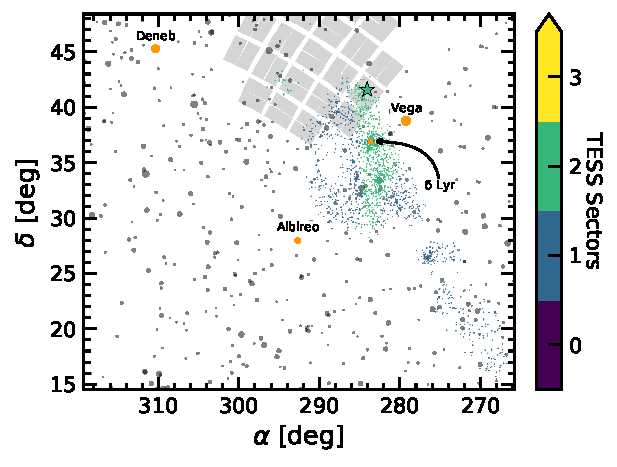
\includegraphics[width=0.48\textwidth]{f2.pdf}
	\end{center}
	\vspace{-0.7cm}
	\caption{
    {\bf Kepler and TESS views of the $\delta$\,Lyr cluster.} Colored
    points are kinematically selected members of the $\delta$\,Lyr
    cluster.  Both Kepler (gray squares) and TESS (colored points)
    observed portions of the cluster.  Naked-eye stars ($m_{\rm
    V}<6.5$) are shown in gray; four of them (orange points) have
    their names annotated.  Kepler\,1627 (green star) was observed
    during the entirety of the Kepler mission, and has been observed
    by TESS for two lunar months to date.
		\label{fig:skychart}
	}
\end{figure}

\begin{figure*}[t]
	\begin{center}
		\leavevmode
		\subfloat{
			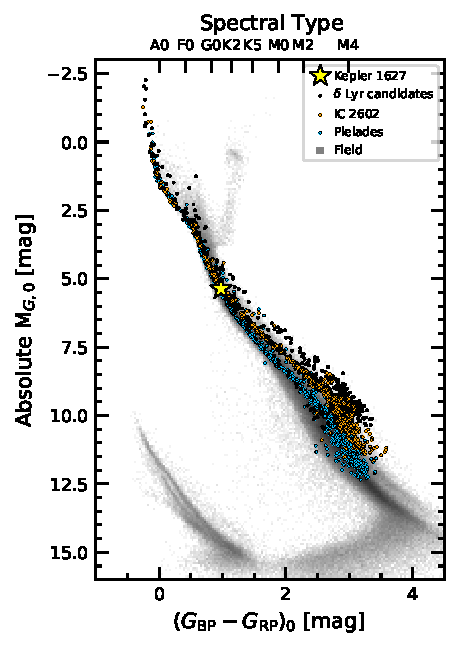
\includegraphics[width=0.49\textwidth]{f15a.pdf}
			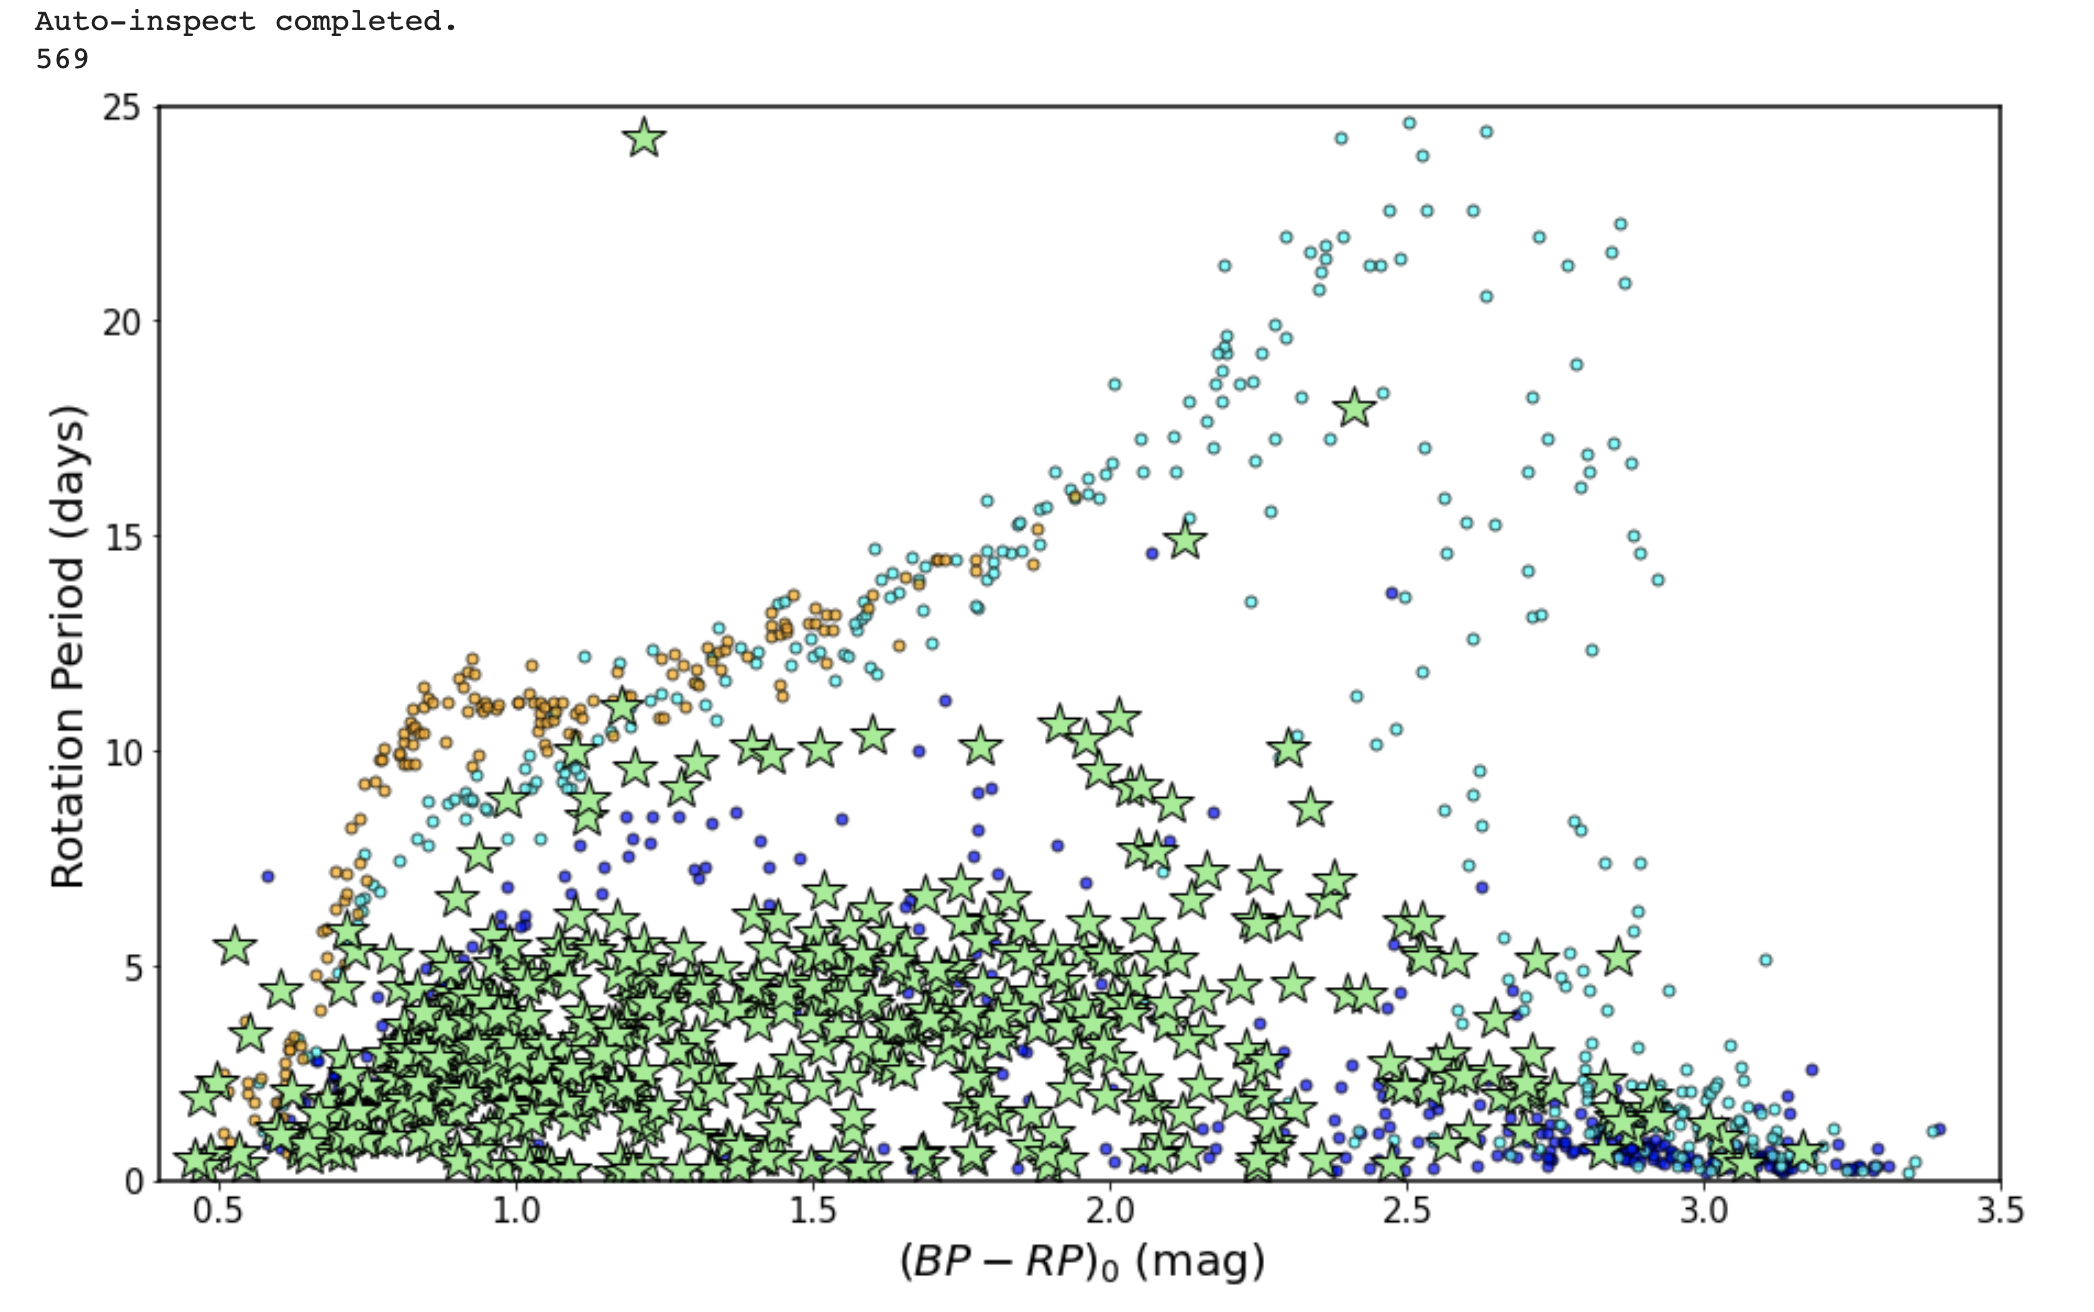
\includegraphics[width=0.49\textwidth]{TEMP_Prot_vs_BpmRp.png}
		}
	\end{center}
	\vspace{-0.7cm}
	\caption{
    {\bf The \cn\ is $35\pm15$\,Myr old.}  {\it Left:} HR diagram of 
    the \cn, IC\,2602 ($\approx35$\,Myr), the Pleiades ($\approx 115$\,Myr), and the field.
    The \cn\ and IC\,2602 are approximately the same isochronal age.
    {\it Right:} TESS and Kepler rotations periods and dereddened Gaia
    colors, with the Pleiades
    \citep[125\,Myr;][]{rebull_rotation_2016a} and Praesepe
    \citep[650\,Myr;][]{douglas_poking_2017} shown for reference.
    Stars of a given color (mass) move up through time due to magnetic
    braking.  The \cn\ has a 40 Myr gyrochronal age, as calibrated
    against the LDB-age of IC\,2602.  {\bf todo: caption improve. fix
    figures.}.
   \label{fig:age}
	}
\end{figure*}

% paragraph 1: HR 
To assess the age of the cluster as well as our star of interest,
we used a combination of the isochronal, gyrochronal, and
lithium-based age-dating.

\subsection{HR Diagram}
We meaured the isochrone age using an empirical approach, and also
compared against theoretical models.
The left panel of Figure~\ref{fig:age} shows the HR diagram of 
stars in the \cn, the Pleiades, IC\,2602, and the field.
The stars shown in the \cn\ are selected based on their positions and
kinematics, as discussed in Appendix~\ref{app:kinematicselection}.
Those from the Pleiades and IC\,2602 are adopted from
\citet{cantatgaudin_gaia_2018}, and the field stars are from the Gaia
EDR3 Catalog of Nearby Stars \citep{gaia_gcns_2021}.
% FIXME FIXME
We corrected for reddening following {\bf procedure X,Y,Z}.

The immediate impression from the left panel of Figure~\ref{fig:age}
is that the \cn\ and IC\,2602 share approximately the same isochronal
age, since they overlap.  In our exploration, we also compared against
$\mu$-Tau ($\approx 60$\,Myr; \citealt{gagne_mutau_2020}) and subsets
of the Sco OB2 association ($\approx10$-$15$\,Myr;
\citealt{damiani_stellar_2019}), and confirmed that the
pre-main-sequence M dwarfs were intermediate between these two
clusters.

% FIXME FIXME
We quantified this impression following the empirical fitting procedure
discussed by \citet{gagne_mutau_2020}.


\subsection{Rotation Periods}
{\bf Jason Curtis todo}
We collected the previously measured
{\bf XXX} Kepler rotation periods (CITEP MCQUILLAN2014), and measured
{\bf YYY} new stellar rotation periods for cluster members observed by
TESS.  We also performed an isochronal analysis.  The results are
shown in Figure~\ref{fig:age}.  From the ensemble perspective, which
provides the strongest constraints (SEE CITET SODERBLOM 2014), the age
of the star is $XX \pm YY$\,Myr.  Individual measurements of the
star's rotation period and lithium abundance corroborate this
conclusion.



\section{The Planet}
\label{sec:planet}

\begin{figure*}[tp]
	\begin{center}
		\leavevmode
		\subfloat{
			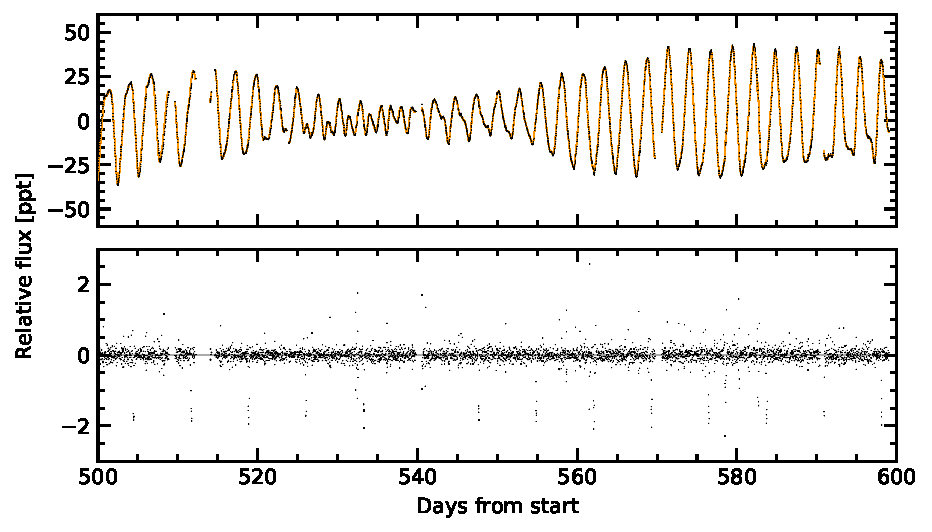
\includegraphics[width=0.9\textwidth]{f4.pdf}
		}
	
		\subfloat{
			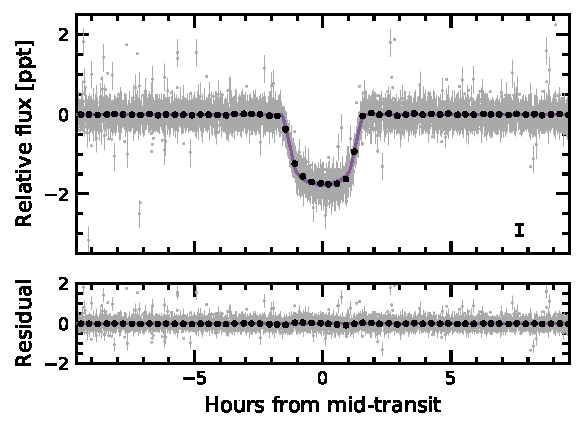
\includegraphics[width=0.87\textwidth]{f5.pdf}
		}
	\end{center}
	\vspace{-0.7cm}
  \caption{ {\bf The light curve of Kepler\,1627.}
    {\it Top}: 
    The full Kepler dataset spans 1{,}437 days (3.9 years), sampled at
    30 minute cadence.  A one hundred day segment is shown here.  The
    {\it top panel} shows the \texttt{PDCSAP} median-subtracted flux
    in units of parts-per-thousand ($\times 10^{-3}$).  The dominant
    signal is induced by starspots.  The model for the stellar
    variability (orange line) is subtracted below, revealing the
    transits of \pn, as well as other deviations from the stellar
    variability model.  The Figure Set available online shows the
    entire 3.9 years of available data.
    {\it Bottom}:
    Phase-folded transit of Kepler 1627b, with stellar variability
    removed.  The 2-$\sigma$ model uncertainties and the maximum {\it
    a posteriori} model are shown as the faint purple band, and the
    dark purple line.  Gray points are individual \texttt{PDCSAP} flux
    measurements; black points are binned to 20 minutes, with a
    representative error bar shown.  The asymmetric residual visible
    during the transit is robust against detrending methods; we
    believe it is caused by starspot crossings.
    \label{fig:lc}
  }
\end{figure*}

\begin{figure}[tp]
	\begin{center}
		\leavevmode
		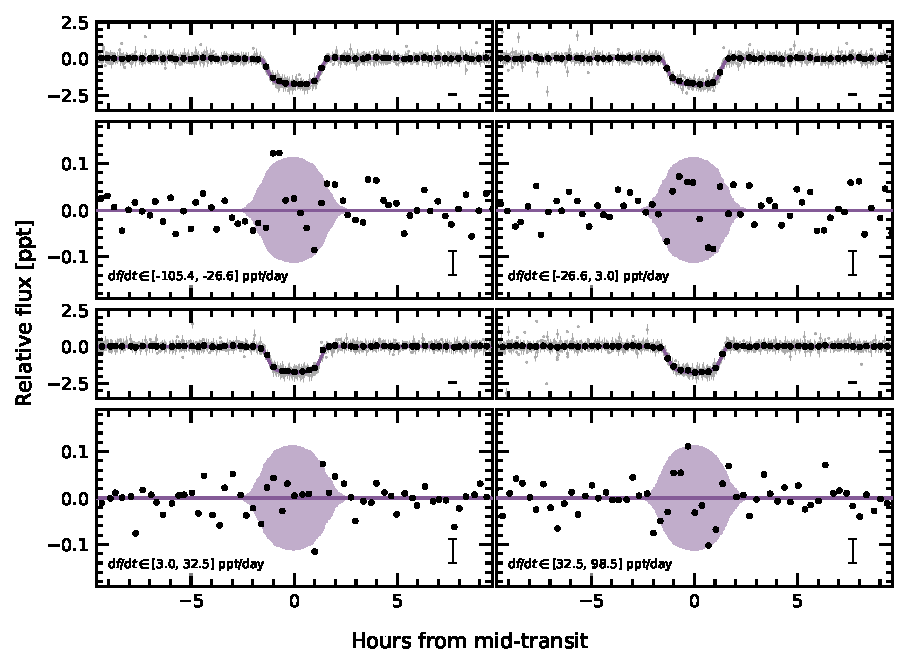
\includegraphics[width=0.48\textwidth]{f11.pdf}
	\end{center}
	\vspace{-0.7cm}
	\caption{
		{\bf Evidence for a prograde orbit from transit timing variations.}
    The time of each transit was measured, along with the local slope
    of the light curve.  The two quantities appear anti-correlated,
    which is most easily explained by starspot crossings during the
    first (second) half of transit inducing a positive (negative) TTV,
    provided that the orbit is prograde \citep{mazeh_time_2015}.  The
    units along the abscissa are most easily understood by considering
    that the flux from the star changes by $\sim$60\,ppt per half
    rotation period ($\sim$1.3\,days).
		\label{fig:ttvslope}
	}
\end{figure}


% rotation period from plot_rotation_period_windowslider.py

If the \pn\ transit signal is created by a bonafide planet, this age
would make it the youngest planet yet found by the main Kepler
mission\footnote{The re-purposed K2 mission found two slightly younger
systems: K2-33b \citep{David_et_al_2017,Mann_K2_33b_2016} and V1298
Tau \citep{david_four_2019}}.  A portion of the light curve is shown
with the phase-folded transit
in Figure~\ref{fig:lc}.  The dominant signal in the
\texttt{PDCSAP} photometry is a quasi-period starspot signal with a
peak-to-peak amplitude that varies between roughly 2\% and 8\%,
depending on the degree of asymmetry in spot coverage between the
stellar hemispheres.  The starspot signal repeats every
$2.642\pm0.042$\,days, where we have adopted an uncertainty based on
the scatter observed between different portions (quarters) of the
time-series data.  The details of how we model this starspot signal to
derive the parameters of the planet are discussed in
Appendix~\ref{app:gptransit}.  The results, given in
Table~\ref{tab:posterior}, are consistent with a mini-Neptune sized
planet ($3.56\pm 0.04\,R_\oplus$) on a circular 7.2\,day orbit
($e<0.XX$), around a G8V star ($0.91 \pm 0.05 R_\odot$).  {\bf TODO
quote the eccentricity limit}

Could the transit signal be produced by anything other than a planet
orbiting this near-solar analog?  \citet{morton_false_2016} considered
the false positive scenarios of a foreground eclipsing binary, a
hierarchical triple-star binary system, and a background eclipsing
binary.  Based on the transit shape, \citet{morton_false_2016} found
the latter scenario to be the only possible case, with a
(model-dependent) probability of $\approx10^{-5}$.  While this
statistical validation is reassuring, ``validated'' planets have been
shown to be false positives \citep{shporer_three_2017}.  Most
failures of the statistical validation approach arise when attempting
to separate the smallest stars from identically-sized gas giant
planets.  With a size of $\approx 3.6\,R_\oplus$, Kepler\,1627b does
not meet this concern.  The fact that we detect a low-mass stellar
companion in archival Keck-NIRC2 Kp-band (2.12\,$\mu $m) imaging does
not change the conclusion: the companion star contributes 1\% of the
flux observed by Kepler.  Combined with the observed transit depth and
shape (Appendix~\ref{app:companionstar}), a planet transiting the
primary star is the only plausible interpretation of the
data.

{\bf todo: LGB to check numbers on full-dataset transit ecc and b} 
Two additional new lines of evidence confirm the planetary
interpretation.  First, the $\approx$100 days of 1-minute
cadenced Kepler observations reduce the cadence-induced smearing,
enabling a more precise measurement of the transit impact parameter
\citep{kipping_binning_2010}.  The planet transits with $b<0.YY$
(3-$\sigma$) from the 1-minute cadenced data, compared to $<0.XX$
(3-$\sigma$) from the 30-minute data.

{\bf todo: Kento to check numbers on per-transit analysis} 
The second line of evidence comes from our transit timing analysis. We
isolated each of the 144 observed transits to within $\pm4.5$\,hr of
each transit, and fitted each window with both {\it i)} a local
second-order polynomial and transit, and {\it ii)} a local linear
trend.  We let the mid-time of each transit float, and then calculated
the residual between the measured mid-time and that of a perfectly
periodic orbit.  This residual, the ``transit timing variation''
(TTV), is plotted in Figure~\ref{fig:ttvslope} against the local
linear slope.  Only a handful of Kepler Objects of Interest have shown
this correlation \citep{holczer_time_2015}, which is most readily
interpreted as a TTV induced by unresolved starspot crossings
\citep{mazeh_time_2015}.  This is of course only possible if the
planet is transiting the primary star, which excludes the any of the
aforementioned false positive scenarios.  It also implies that the
planet's orbit is prograde.  The latter interpretation assumes that
the dominant photometric variability is induced by dark spots, rather
than bright faculae.  Given the observed transition of Sun-like
stellar variability from spot to faculae-dominated regimes, we expect
this inference to be reasonably secure
\citep{shapiro_are_2016,montet_long-term_2017,reinhold_stellar_2020}.

\section{Discussion \& Conclusions}
\label{sec:conc}

\begin{figure*}[tp]
	\begin{center}
		\leavevmode
		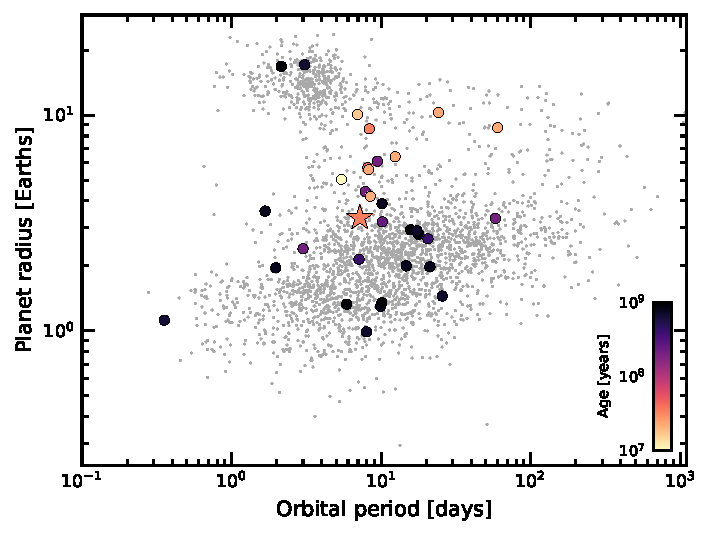
\includegraphics[width=\textwidth]{f14.pdf}
	\end{center}
	\vspace{-0.7cm}
	\caption{
    {\bf Radii, orbital periods, and ages of known transiting
    exoplanets}.  Planets older than
    $10^9$ years are shown with gray markers.  Planets younger than a
    gigayear, with $t/\sigma_t > 3$, are shown in color.  
    \pn\ is shown with a star.
    The abnormally large radii of the youngest transiting planets
    could be explained by their primordial atmospheres not yet
    having evaporated.
    Selection effects could also be important.
    Parameters were acquired from the NASA Exoplanet Archive on July
    2, 2021.
		\label{fig:rp_period_age}
	}
\end{figure*}


{\bf LGB TODO: ask James Owen what he thinks the mass loss rate is}
Kepler\,1627Ab therefore provides a new extremum in the ages of the
Kepler planets, and opens multiple avenues for study from the ground.
Observations of its Doppler transit are expected to induce a
Rossiter-McLaughlin anomaly with an amplitude of $\approx 20$\ms, and
could yield a quantification of the stellar obliquity, and a means for
verifying our transit-timing based suggestion of a prograde orbit.
Similar transit spectroscopy aimed at detecting either hydrogen or
helium absorption could yield insight into the planet's atmosphere,
which is expected to be outflowing at a rate of {\bf
X.X}\,$M_\oplus\,{\rm yr}^{-1}$ (CITE).  A more challenging
measurement would be a measurement of the planet's mass, through
either detailed timing analyses of the Kepler data, or through a
high-cadence multi-color radial velocity campaign.  The mass could
yield constraints on both the planet's composition as well as its
initial entropy \citep{owen_constraining_2020}.

The precision of the Kepler data itself may enable more detailed
analyses without needing to acquire more data.  While our transit
timing study did not yield the detection of any clearly significant
planet-planet induced TTVs, the star's flaring may be suggestive of
star-planet interactions.  Appendix~\ref{app:flare} highlights an odd
flare timing coincidence that may be worthy of further examination.

In the context of the known transiting planets, \pn\ is among the
youngest known (Figure~\ref{fig:rp_period_age}).  Comparable systems
with precisely measured ages spanning 10 to 100\,Myr include K2-33b,
DS~Tuc~Ab, HIP~67522b, TOI~837b, AU~Mic~b, and the four-planet
V1298~Tau system
\citep{Mann_K2_33b_2016,David_et_al_2017,newton_tess_2019,david_four_2019,bouma_cluster_2020,plavchan_planet_2020}.
Of these systems, \pn\ inhabits a similar range of planetary size and
orbital period.  It is the smallest though ($3.6\,R_\oplus$), which
may hint at selection effects in the sample of young planets
\citep{zhou_2021_tois}.  Assuming that these planets have masses
between $\approx$10 and 20$\,M_\oplus$, their large sizes and presumed
low densities are in accord with the expectation that mini-Neptunes
start their lives with large primordial atmopsheres that are are lost
over the first gigayear
\citep{Owen_Wu_2013,Fulton_et_al_2017,ginzburg_corepowered_2018}.
The observation from starspot-induced TTVs that the planetary orbit
could be aligned with the stellar spin differs from a number of other
close-in
mini-Neptunes~\citep{sanchis-ojeda_starspots_2011,albrecht_obliquities_2012,dalal_2019_hd3167,rubenzahl_tess-keck_2021}.
Overall however, it is consistent with a quiescent disk-driven
migration history for the planet, while the in-situ formation scenario
is disfavored because the necessary disk mass would always drive
planets to migrate
\citep{inamdar_formation_2015,ogihara_reassessment_2015}.


% TODO: decide whether a paragraph about young planet obliquities is
% needed.

% The orbits of the planets can also change early on, and can become
% significantly misaligned from the equators of their host stars.
% Measurements of the sky-projected angle between the planet orbit and
% the stellar spin (the stellar obliquity) have shown that high
% obliquities characterize hot field stars hosting both hot Jupiters and
% smaller planets \citep{winn10,louden21}.  Conversely, the obliquities
% of planets around cool stars tend to be low, but this could be due to
% tidal realignment \citep[{\it e.g.},][]{anderson21}.  Obliquity
% measurements for young planets are therefore important, because they
% provide an unobstructed view of the primordial obliquity distribution. 



Ultimately, our age measurement for \pn\ was enabled by identifying
its connection to the \cn\ using the Gaia data.  The Supplementary
Table~\ref{tab:v05} enables similar crossmatches to already known
planets, as well as forthcoming planets from the TESS mission
\citep{ricker_transiting_2015,guerrero_tess_2021}.  An alternative
approach would be to identify kinematic associations around exoplanet
host stars using the Gaia data, and to then verify these associations
with ancilliary rotation periods and spectroscopy
\citep{tofflemire_tess_2021}.


%%%%%%%%%%%%%%%%%%%%%%%%%%%%%%%%%%%%%%%%%%%%%%%%%%%%%%%%%%%%%%%%%%%%%%%%%%%%%%%


% Table of best fit parameters
%\startlongtable
\begin{deluxetable*}{lllrrrrrrr}
%
  \tablecaption{ Priors and posteriors for the transit and stellar
  variability model fitted to the long-cadence Kepler 1627b
  photometric timeseries.}
\label{tab:posterior}
%
\tabletypesize{\scriptsize}
%\tabletypesize{\small}
%
%\tablenum{2}
%
\tablehead{
  \colhead{Param.} & 
  \colhead{Unit} &
  \colhead{Prior} & 
  \colhead{Median} & 
  \colhead{Mean} & 
  \colhead{Std{.} Dev.} &
  \colhead{3\%} &
  \colhead{97\%} &
  \colhead{ESS} &
  \colhead{$\hat{R}-1$}
}

%/Users/luke/Dropbox/proj/rudolf/results/run_RotStochGPtransit/Kepler_1627_RotStochGPtransit_posteriortable.tex
\startdata
{\it Sampled} & & & & & & & & & \\
\hline
$P$ & d & $\mathcal{N}(7.20281; 0.01000)$ & 7.2028035 & 7.2028033 & 0.0000073 & 7.2027893 & 7.2028171 & 1910.5903732 & 0.0035905 \\
$t_0^{(1)}$ & d & $\mathcal{N}(120.79053; 0.02000)$ & 120.790504 & 120.790505 & 0.0009438 & 120.7886867 & 120.7922431 & 1564.1105056 & 0.0003213 \\
$\log R_{\rm p}/R_\star$ & -- & $\mathcal{U}(-4.605; 0.000)$ & -3.33523 & -3.33569 & 0.06618 & -3.45772 & -3.21617 & 1173.56574 & 0.00310 \\
$b$ & -- & $\mathcal{U}(0; 1+R_{\mathrm{p}}/R_\star)$ & 0.3971 & 0.3886 & 0.2070 & 0.0204 & 0.7289 & 378.9528 & 0.0177 \\
$u_1$ & -- & \citet{exoplanet:kipping13} & 0.28 & 0.30 & 0.179 & 0.002 & 0.603 & 1161.95 & 0.005 \\
$u_2$ & -- & \citet{exoplanet:kipping13} & 0.425 & 0.381 & 0.314 & -0.197 & 0.912 & 900.884 & 0.002 \\
$R_\star$ & $R_\odot$ & $\mathcal{T}(0.910; 0.052)$ & 0.911 & 0.910 & 0.051 & 0.814 & 1.004 & 2265.830 & -0.001 \\
$\log g$ & cgs & $\mathcal{N}(4.600; 0.100)$ & 4.604 & 4.601 & 0.094 & 4.417 & 4.769 & 923.943 & 0. \\
$\langle f \rangle$ & -- & $\mathcal{N}(0.500; 0.100)$ & 0.4999 & 0.4999 & 0.0003 & 0.4993 & 0.5005 & 2964.6676 & 0.0013 \\
$e^{(2)}$ & -- & \citet{vaneylen19} & 0.127 & 0.168 & 0.147 & 0. & 0.446 & 518.492 & 0.004 \\
$\omega$ & rad & $\mathcal{U}(0.000; 6.283)$ & -0.235 & -0.170 & 1.867 & -2.879 & 3.132 & 1212.260 & 0.006 \\
$\log \sigma_f$ & -- & $\mathcal{N}(\log\langle \sigma_f \rangle; 2.000)$ & -8.016 & -8.016 & 0.008 & -8.031 & -8.001 & 2224.427 & -0. \\
$\rho$ & d & $\mathcal{U}(1.000; 10.000)$ & 2.953 & 2.955 & 0.096 & 2.777 & 3.131 & 1936.492 & 0. \\
$\sigma$ & d$^{-1}$ & $\mathrm{InvGamma}(1.000; 5.000)$ & 0.013 & 0.013 & 0.001 & 0.012 & 0.014 & 2155.687 & -0. \\
$\sigma_{\mathrm{rot}}$ & d$^{-1}$ & $\mathrm{InvGamma}(1.000; 5.000)$ & 0.897 & 0.933 & 0.222 & 0.552 & 1.316 & 2147.324 & 0.003 \\
$\log P_{\mathrm{rot}}$ & $\log (\mathrm{d})$ & $\mathcal{N}(0.958; 0.020)$ & 0.964 & 0.964 & 0.001 & 0.963 & 0.966 & 2486.029 & 0. \\
$\log Q_0$ & -- & $\mathcal{N}(0.000; 2.000)$ & 12.935 & 12.960 & 0.454 & 12.157 & 13.857 & 2126.581 & 0.004 \\
$\log \mathrm{d}Q$ & -- & $\mathcal{N}(0.000; 2.000)$ & 0.029 & 0.021 & 2.032 & -3.785 & 3.780 & 1755.941 & 0. \\
$f$ & -- & $\mathcal{U}(0.100; 1.000)$ & 0.111 & 0.113 & 0.010 & 0.1 & 0.130 & 1253.358 & -0.0 \\
\hline
{\it Derived} & & & & & & & & & \\
\hline
$R_{\rm p}/R_\star$ & -- & -- & 0.036 & 0.036 & 0.002 & 0.031 & 0.040 & 1173.566 & 0.003 \\
$\rho_\star$ & g$\ $cm$^{-3}$ & -- & 2.27 & 2.312 & 0.516 & 1.408 & 3.272 & 910.746 & 0.001 \\
$R_{\rm p}$ & $R_{\mathrm{Jup}}$ & -- & 0.316 & 0.317 & 0.037 & 0.251 & 0.386 & 1692.736 & 0.001 \\
$a/R_\star$ & -- & -- & 18.396 & 18.407 & 1.375 & 15.690 & 20.780 & 910.717 & 0.001 \\
$\cos i$ & -- & -- & 0.022 & 0.021 & 0.011 & 0.002 & 0.038 & 439.303 & 0.011 \\
$T_{14}$ & hr & -- & 2.822 & 2.823 & 0.057 & 2.710 & 2.917 & 1086.008 & 0.002 \\
$T_{13}$ & hr & -- & 2.578 & 2.566 & 0.083 & 2.430 & 2.714 & 590.630 & 0.011 \\
\enddata
%
\tablecomments{
  ESS refers to the number of effective samples.
  $\hat{R}$ is the Gelman-Rubin convergence diagnostic.
  Logarithms through this table are in base-$e$.
  $\mathcal{U}$ denotes a uniform distribution,
  $\mathcal{N}$ a normal distribution, and
  $\mathcal{T}$ a truncated normal bounded between zero and an upper limit much larger than the mean.
  (1) The ephemeris is in units of BJDTDB - 2454833.
  (2) The eccentricity vectors are sampled in the $(e\cos\omega,
  e\sin\omega)$ basis.
%
% (2) Uninformative quadratic limb-darkening prior from \citet{exoplanet:kipping13}, implemented by \citet{exoplanet:exoplanet}.
% The precision achieved in the ground-based data did not appear to
% necessitate using bandpass-dependent limb-darkening coefficients.
% For comparison, the \citet{claret_limb_2017} parameters for
% the appropriate $T_{\rm eff}$ and $\log g$ in TESS-band would have been 
% $(u_1, u_2) = (0.3249, 0.235)$.
%
% (2) Assuming an informative quadratic limb-darkening prior with
% values about those given for the appropriate $T_{\rm eff}$ and
% $\log g$ in TESS-band from \citet{claret_limb_2017}. The precision
% achieved in the ground-based data did not appear to necessitate using
% bandpass-dependent limb-darkening coefficients.
% (3) The second and third contact points do not exist for a grazing transit.
% {\it Notation}:
% $a_{ij;\mathrm{Instr}}$ denotes the $i^{\rm th}$ transit of a
% particular instrument, and the $j^{\rm th}$ polynomial detrending
% order.
}
\vspace{-0.3cm}
\end{deluxetable*}



%\clearpage
\acknowledgements
\raggedbottom

L.G.B{.} and J.L.C{.} are grateful to T{.}~David for help with the
transit fitting, to R{.}~Kerr for kindly providing us with the
\citet{kerr_stars_2021} membership list prior to its publication.
% is grateful to G.~Zhou, B{.}~Tofflemire, A{.}~McWilliam,
% E{.}~Newton, M{.}~Kounkel, A{.}~Kraus, L{.}~Hillenbrand, and
% K{.}~Hawkins for the discussions on young stars, rotation, and lithium
% that encouraged this analysis.
%
L.G.B{.} acknowledges support by the TESS GI Program, programs
G011103 and G022117, through NASA grants 80NSSC19K0386 and
80NSSC19K1728.
%
L.G.B{.} was also supported by a Charlotte Elizabeth Procter
Fellowship from Princeton University.
%
This study was based in part on observations at Cerro Tololo
Inter-American Observatory at NSF's NOIRLab (NOIRLab Prop{.} ID
2020A-0146; 2020B-0029 PI: Bouma), which is managed by the
Association of Universities for Research in Astronomy (AURA) under a
cooperative agreement with the National Science Foundation.
%
% ACKNOWLEDGE PFS / CAMPANAS.
%
This paper also includes data collected by the TESS mission, which are
publicly available from the Mikulski Archive for Space Telescopes
(MAST).
%
Funding for the TESS mission is provided by NASA's Science Mission
directorate.
%
We thank the TESS Architects (G.~Ricker, R.~Vanderspek, D.~Latham,
S.~Seager, J.~Jenkins) and the many TESS team members for their
efforts to make the mission a continued success.
%

%
% The Digitized Sky Survey was produced at the Space Telescope Science
% Institute under U.S. Government grant NAG W-2166.
% Figure~\ref{fig:scene} is based on photographic data obtained using
% the Oschin Schmidt Telescope on Palomar Mountain.
%

% %
% This research made use of the NASA Exoplanet Archive, which is
% operated by the California Institute of Technology, under contract
% with the National Aeronautics and Space Administration under the
% Exoplanet Exploration Program.
% %

% Resources supporting this work were provided by the NASA High-End
% Computing (HEC) Program through the NASA Advanced Supercomputing (NAS)
% Division at Ames Research Center for the production of the SPOC data
% products.
%

% A.J.\ and R.B.\ acknowledge support from project IC120009 ``Millennium
% Institute of Astrophysics (MAS)'' of the Millenium Science Initiative,
% Chilean Ministry of Economy. A.J.\ acknowledges additional support
% from FONDECYT project 1171208.  J.I.V\ acknowledges support from
% CONICYT-PFCHA/Doctorado Nacional-21191829.  R.B.\ acknowledges support
% from FONDECYT Post-doctoral Fellowship Project 3180246.
% %
% C.T.\ and C.B\ acknowledge support from Australian Research Council
% grants LE150100087, LE160100014, LE180100165, DP170103491 and
% DP190103688.
% %
% C.Z.\ is supported by a Dunlap Fellowship at the Dunlap Institute for
% Astronomy \& Astrophysics, funded through an endowment established by
% the Dunlap family and the University of Toronto.
% %
% D.D.\ acknowledges support through the TESS Guest Investigator Program
% Grant 80NSSC19K1727.
%
%
%
% %
% Based on observations obtained at the Gemini Observatory, which is
% operated by the Association of Universities for Research in Astronomy,
% Inc., under a cooperative agreement with the NSF on behalf of the
% Gemini partnership: the National Science Foundation (United States),
% National Research Council (Canada), CONICYT (Chile), Ministerio de
% Ciencia, Tecnolog\'{i}a e Innovaci\'{o}n Productiva (Argentina),
% Minist\'{e}rio da Ci\^{e}ncia, Tecnologia e Inova\c{c}\~{a}o (Brazil),
% and Korea Astronomy and Space Science Institute (Republic of Korea).
% %
% Observations in the paper made use of the High-Resolution Imaging
% instrument Zorro at Gemini-South. Zorro was funded by the NASA
% Exoplanet Exploration Program and built at the NASA Ames Research
% Center by Steve B. Howell, Nic Scott, Elliott P. Horch, and Emmett
% Quigley.
% %
% This research has made use of the VizieR catalogue access tool, CDS,
% Strasbourg, France. The original description of the VizieR service was
% published in A\&AS 143, 23.
% %
% This work has made use of data from the European Space Agency (ESA)
% mission {\it Gaia} (\url{https://www.cosmos.esa.int/gaia}), processed
% by the {\it Gaia} Data Processing and Analysis Consortium (DPAC,
% \url{https://www.cosmos.esa.int/web/gaia/dpac/consortium}). Funding
% for the DPAC has been provided by national institutions, in particular
% the institutions participating in the {\it Gaia} Multilateral
% Agreement.
%
% (Some of) The data presented herein were obtained at the W. M. Keck
% Observatory, which is operated as a scientific partnership among the
% California Institute of Technology, the University of California and
% the National Aeronautics and Space Administration. The Observatory was
% made possible by the generous financial support of the W. M. Keck
% Foundation.
% The authors wish to recognize and acknowledge the very significant
% cultural role and reverence that the summit of Maunakea has always had
% within the indigenous Hawaiian community.  We are most fortunate to
% have the opportunity to conduct observations from this mountain.
%
% \newline
%

\software{
  %\texttt{arviz} \citep{arviz_2019},
  \texttt{astrobase} \citep{bhatti_astrobase_2018},
  %\texttt{astroplan} \citep{astroplan2018},
	%\texttt{AstroImageJ} \citep{collins_astroimagej_2017},
  \texttt{astropy} \citep{astropy_2018},
  \texttt{astroquery} \citep{astroquery_2018},
  %\texttt{BATMAN} \citep{kreidberg_batman_2015},
  %\texttt{ceres} \citep{brahm_2017_ceres},
  %\texttt{cdips-pipeline} \citep{bhatti_cdips-pipeline_2019},
  \texttt{corner} \citep{corner_2016},
  %\texttt{emcee} \citep{foreman-mackey_emcee_2013},
  \texttt{exoplanet} \citep{exoplanet:exoplanet}, and its
  dependencies \citep{exoplanet:agol20, exoplanet:kipping13, exoplanet:luger18,
   	exoplanet:theano},
	%\texttt{gala} \citep{gala,PriceWhelan_2017_gala_zenodo},
	%\texttt{IDL Astronomy User's Library} \citep{landsman_1995},
  \texttt{IPython} \citep{perez_2007},
	%\texttt{isochrones} \citep{morton_2015_isochrones},
	%\texttt{lightkurve} \citep{lightkurve_2018},
  \texttt{matplotlib} \citep{hunter_matplotlib_2007}, 
  %\texttt{MESA} \citep{paxton_modules_2011,paxton_modules_2013,paxton_modules_2015}
  \texttt{numpy} \citep{walt_numpy_2011}, 
  \texttt{pandas} \citep{mckinney-proc-scipy-2010},
  %\texttt{pyGAM} \citep{serven_pygam_2018_1476122},
  \texttt{PyMC3} \citep{salvatier_2016_PyMC3},
  %\texttt{radvel} \citep{fulton_radvel_2018},
  %\texttt{scikit-learn} \citep{scikit-learn},
  \texttt{scipy} \citep{jones_scipy_2001},
  \texttt{TESS-point}  \citep{burke_2020},
  %\texttt{tesscut} \citep{brasseur_astrocut_2019},
	%\texttt{VESPA} \citep{morton_efficient_2012,vespa_2015},
  %\texttt{webplotdigitzer} \citep{rohatgi_2019},
  \texttt{wotan} \citep{hippke_wotan_2019}.
}
\ 

\facilities{
 	{\it Astrometry}:
 	Gaia \citep{gaia_collaboration_gaia_2018,gaia_collaboration_2020_edr3}.
 	{\it Imaging}:
    Second Generation Digitized Sky Survey. %,
    %SOAR~(HRCam; \citealt{tokovinin_ten_2018}).
 	%Keck:II~(NIRC2; \url{www2.keck.hawaii.edu/inst/nirc2}).
 	%Gemini:South~(Zorro; \citealt{scott_nessi_2018}.
 	{\it Spectroscopy}:
	CTIO1.5$\,$m~(CHIRON; \citealt{tokovinin_chironfiber_2013}),
  %PFS ({\bf CITE}),
  %  MPG2.2$\,$m~(FEROS; \citealt{kaufer_commissioning_1999}),
	%AAT~(Veloce; \citealt{gilbert_veloce_2018}).
	AAT~(HERMES; \citealt{lewis_2002_hermers_2df,sheinis_2015_hermes}),
 	%Keck:I~(HIRES; \citealt{vogt_hires_1994}).
 	VLT:Kueyen~(FLAMES; \citealt{pasquini_2002}).
% 	Euler1.2m~(CORALIE),
% 	ESO:3.6m~(HARPS; \citealt{mayor_setting_2003}).
 	{\it Photometry}:
%	  ASTEP:0.40$\,$m (ASTEP400),
% 	CTIO:1.0m (Y4KCam),
% 	Danish 1.54m Telescope,
%	  El Sauce:0.356$\,$m,
% 	Elizabeth 1.0m at SAAO,
% 	Euler1.2m (EulerCam),
	  Kepler \citep{borucki_kepler_2010},
% 	Magellan:Baade (MagIC),
% 	Max Planck:2.2m	(GROND; \citealt{greiner_grond7-channel_2008})
% 	NTT,
% 	SOAR (SOI),
 	TESS \citep{ricker_transiting_2015}.
% 	TRAPPIST \citep{jehin_trappist_2011},
% 	VLT:Antu (FORS2).
}

% \input{TOI837_phot_table.tex}
% \input{TOI837_rv_table.tex}
% \input{ic2602_ages.tex}
% \begin{table*}
\scriptsize
\setlength{\tabcolsep}{2pt}
\centering
\caption{Literature and Measured Properties for Kepler$\,$1627}
\label{tab:starparams}
%\tablenum{2}
\begin{tabular}{llcc}
  \hline
  \hline
Primary Star\dotfill & \\
\multicolumn{3}{c}{TIC 120105470} \\
\multicolumn{3}{c}{GAIADR2$^\dagger$ 2103737241426734336} \\
\hline
\hline
Parameter & Description & Value & Source\\
\hline 
$\alpha_{J2015.5}$\dotfill	&Right Ascension (hh:mm:ss)\dotfill & 18:56:13.6 & 1	\\
$\delta_{J2015.5}$\dotfill	&Declination (dd:mm:ss)\dotfill & +41:34:36.22 & 1	\\
%
V\dotfill			&Johnson V mag.\dotfill & 13.11 $\pm$ 0.08		& 2	\\
${\rm G}$\dotfill     & Gaia $G$ mag.\dotfill     & 13.02$\pm$0.02 & 1\\
$G_{\rm BP}$\dotfill     & Gaia $BP$ mag.\dotfill     & 13.43$\pm$0.02 & 1\\
$G_{\rm RP}$\dotfill     & Gaia $RP$ mag.\dotfill     & 12.44$\pm$0.02 & 1\\
${\rm T}$\dotfill     & TESS $T$ mag.\dotfill     & 12.53$\pm$0.02 & 2\\
J\dotfill			& 2MASS J mag.\dotfill & 11.69  $\pm$ 0.02	& 3	\\
H\dotfill			& 2MASS H mag.\dotfill & 11.30 $\pm$ 0.02	    &  3	\\
K$_{\rm S}$\dotfill			& 2MASS ${\rm K_S}$ mag.\dotfill & 11.19 $\pm$ 0.02 &  3	\\
%
$\pi$\dotfill & Gaia EDR3 parallax (mas) \dotfill & 3.009 $\pm$ 0.032 &  1 \\
$d$\dotfill & Distance (pc)\dotfill & $329.5 \pm 3.5$ & 1, 4 \\
$\mu_{\alpha}$\dotfill		& Gaia EDR3 proper motion\dotfill & 1.716 $\pm$ 0.034 & 1 \\
                    & \hspace{3pt} in RA (mas yr$^{-1}$)	&  \\
$\mu_{\delta}$\dotfill		& Gaia EDR3 proper motion\dotfill 	&  -1.315 $\pm$ 0.034 &  1 \\
                    & \hspace{3pt} in DEC (mas yr$^{-1}$) &  \\
RUWE\dotfill		& Gaia EDR3 renormalized\dotfill 	&  2.899 &  1 \\
                    & \hspace{3pt} unit weight error &  \\
RV\dotfill & Systemic radial \hspace{9pt}\dotfill  & $-16.7 \pm 1.0$ & 5 \\
                    & \hspace{3pt} velocity (\kms)  & \\
%
Spec. Type\dotfill & Spectral Type\dotfill & 	G8V & 5 \\
$v\sin{i_\star}$\dotfill &  Rotational velocity$^*$ (\kms) \hspace{9pt}\dotfill &  18.9 $\pm$ 1.0 & 5 \\
Li EW\dotfill & 6708\AA\ Equiv{.} Width (m\AA) \dotfill & $233^{+5}_{-7}$  & 5 \\
$T_{\rm eff}$\dotfill &  Effective Temperature (K) \hspace{9pt}\dotfill & 5505 $\pm$ 60 &  6  \\
$\log{g_{\star}}$\dotfill &  Surface Gravity (cgs)\hspace{9pt}\dotfill &  4.53 $\pm$ 0.05  &  6 \\
$R_\star$\dotfill & Stellar radius ($R_\odot$)\dotfill & 0.881$\pm$0.018 & 6 \\
$M_\star$\dotfill & Stellar mass ($R_\odot$)\dotfill & 0.953$\pm$0.019 & 6 \\
$A_{\rm V}$\dotfill & Interstellar reddening (mag)\dotfill & 0.2 $\pm$ 0.1 & 6 \\
${\rm [Fe/H]}$\dotfill &   Metallicity\dotfill & 0.1 $\pm$ 0.1 & 6 \\
%
$P_{\rm rot}$\dotfill & Rotation period (d)\dotfill & $2.642\pm 0.042$  & 7 \\
Age & Adopted stellar age (Myr)\dotfill & $38^{+6}_{-5}$  &  8 \\
%
\hline 
%
$\Delta m_{832}$ & Mag difference (`Alopeke 832\,nm)\dotfill & $3.14 \pm 0.04$ & 9 \\
$\theta_{\rm B}$ & Position angle (deg)\dotfill & $91.9 \pm 0.7$ & 9 \\
$\rho_{\rm B}$ & Apparent separation of \dotfill & $0.164 \pm 0.010$ &  9 \\
                    & \hspace{3pt} primary and secondary (as) &  \\
$\rho_{\rm B}$ & Apparent separation of \dotfill & $53 \pm 4$ &  1,4,9 \\
                    & \hspace{3pt} primary and secondary (AU) &  \\
$\Delta m_{K'}$ & Mag difference (NIRC2 $K'$)\dotfill & $2.37 \pm 0.02$ & 10 \\
$\theta_{\rm B}$ & Position angle (deg)\dotfill & $95.9 \pm 0.5$ & 10 \\
$\rho_{\rm B}$ & Apparent separation of \dotfill & $0.1739 \pm 0.0017$ &  10 \\
                    & \hspace{3pt} primary and secondary (as) &  \\
%
\hline
\end{tabular}
\begin{flushleft}
 \footnotesize{ \textsc{NOTE}---
 $^\dagger$ The GAIADR2 and GAIAEDR3 identifiers for Kepler 1627A are identical.  The secondary
 is not resolved in the Gaia point source catalog.
 $^*$ Given only $v\sin i$ and $2\piR_\star/P_{\rm rot}$, $\cos i=0.11^{+0.11}_{-0.08}$.
Provenances are:
$^1$\citet{gaia_collaboration_2021_edr3},
$^2$\citet{stassun_TIC8_2019},
$^3$\citet{skrutskie_tmass_2006},
$^4$\citet{Lindegren_2021_offset},
$^5$HIRES spectra and \citet{yee_SM_2017},
$^6$Cluster isochrone (MIST adopted; PARSEC compared for quoted
  uncertainty),
$^7$Kepler light curve,
$^8$Pre-main-sequence CAMD interpolation (Section~\ref{sec:camd}),
$^9$`Alopeke imaging 2021 June 24 \citep{scott_twin_2021},
$^{10}$NIRC2 imaging 2015 July 22.
}
\end{flushleft}
\vspace{-0.5cm}
\end{table*}

% \input{compparams.tex}


\clearpage
\bibliographystyle{yahapj}                            
\bibliography{bibliography} 

\appendix
\section{Young, Age-Dated, and Age-Dateable Star Compilation}
\label{app:targetlist}

%% \begin{deluxetable}{} command tell LaTeX how many columns
%% there are and how to align them.
%\startlongtable
\begin{deluxetable*}{lll}
    
%% Keep a portrait orientation

%% Over-ride the default font size
%% Use Default (12pt)
\tabletypesize{\scriptsize}
%\tabletypesize{\small}

%% Use \tablewidth{?pt} to over-ride the default table width.
%% If you are unhappy with the default look at the end of the
%% *.log file to see what the default was set at before adjusting
%% this value.

%% This is the title of the table.
\tablecaption{Young, Age-dated, and Age-dateable Stars Within the
  Nearest Few Kiloparsecs ($\texttt{v0.5}$ of the CDIPS Target
  List).}
\label{tab:v05}

%% This command over-rides LaTeX's natural table count
%% and replaces it with this number.  LaTeX will increment 
%% all other tables after this table based on this number
%\tablenum{3}

%% The \tablehead gives provides the column headers.  It
%% is currently set up so that the column labels are on the
%% top line and the units surrounded by ()s are in the 
%% bottom line.  You may add more header information by writing
%% another line between these lines. For each column that requries
%% extra information be sure to include a \colhead{text} command
%% and remember to end any extra lines with \\ and include the 
%% correct number of &s.
\tablehead{
  \colhead{Parameter} &
  \colhead{Example Value} &
  \colhead{Description}
}

%% All data must appear between the \startdata and \enddata commands
%
% paste from
% /Users/luke/Dropbox/proj/rudolf/results/tables/v05_main_tableheader.tex
% via drivers/write_v05_main_tableheader.py
\startdata
         \texttt{source\_id} &                                         1709456705329541504 &                                             Gaia DR2 source identifier. \\
                 \texttt{ra} &                                                     247.826 &                                         Gaia DR2 right ascension [deg]. \\
                \texttt{dec} &                                                      79.789 &                                             Gaia DR2 declination [deg]. \\
           \texttt{parallax} &                                                      35.345 &                                                Gaia DR2 parallax [mas]. \\
    \texttt{parallax\_error} &                                                       0.028 &                                    Gaia DR2 parallax uncertainty [mas]. \\
               \texttt{pmra} &                                                      94.884 &     Gaia DR2 proper motion $\mu_\alpha \cos \delta$ [mas$\,$yr${^-1}$]. \\
              \texttt{pmdec} &                                                     -86.971 &                 Gaia DR2 proper motion $\mu_\delta$ [mas$\,$yr${^-1}$]. \\
 \texttt{phot\_g\_mean\_mag} &                                                        6.85 &                                                 Gaia DR2 $G$ magnitude. \\
\texttt{phot\_bp\_mean\_mag} &                                                       6.409 &                                     Gaia DR2 $G_\mathrm{BP}$ magnitude. \\
\texttt{phot\_rp\_mean\_mag} &                                                       7.189 &                                     Gaia DR2 $G_\mathrm{RP}$ magnitude. \\
            \texttt{cluster} &                 Uma,IR\_excess,NASAExoArchive\_ps\_20210506 &                                  Comma-separated cluster or group name. \\
                \texttt{age} &                                                nan,nan,9.48 & Comma-separated logarithm (base-10) of reported$^{\rm a}$ age in years. \\
          \texttt{mean\_age} &                                                        9.48 &                          Mean (ignoring NaNs) of $\texttt{age}$ column. \\
      \texttt{reference\_id} &      Ujjwal2020,CottenSong2016,NASAExoArchive\_ps\_20210506 &                          Comma-separted provenance of group membership. \\
 \texttt{reference\_bibcode} & 2020AJ....159..166U,2016ApJS..225...15C,2013PASP..125..989A &                  ADS bibcode corresponding to $\texttt{reference\_id}$. \\
\enddata

%% Include any \tablenotetext{key}{text}, \tablerefs{ref list},
%% or \tablecomments{text} between the \enddata and 
%% \end{deluxetable} commands

%% General table comment marker
\tablecomments{
Table~\ref{tab:v05} is
published in its entirety in a machine-readable format.   This table is a
concatenation of the studies listed in Table~\ref{tab:metadata}.
One entry is
shown for guidance regarding form and content. 
In this particular example, the star has a
cold Jupiter on a 16 year orbit, HD 150706b \citep{2012AA...545A..55B}.
An infrared excess has been reported \citep{CottenSong2016}, and the star was identified by \citet{Ujjwal2020} as a candidate UMa moving group
member ($\approx 400\,{\rm Myr}$; \citealt{mann_tess_2020}).
The star's RV activity and TESS rotation period corroborate its youth.
}
\vspace{-0.5cm}
\end{deluxetable*}

%% \begin{deluxetable}{} command tell LaTeX how many columns
%% there are and how to align them.
%\startlongtable
\begin{deluxetable*}{lccc}
    
%% Keep a portrait orientation

%% Over-ride the default font size
%% Use Default (12pt)
\tabletypesize{\scriptsize}
%\tabletypesize{\small}
%\tabletypesize{\normal}

%% Use \tablewidth{?pt} to over-ride the default table width.
%% If you are unhappy with the default look at the end of the
%% *.log file to see what the default was set at before adjusting
%% this value.

%% This is the title of the table.
\tablecaption{Provenances of Young and Age-dateable Stars.}
\label{tab:metadata}

%% This command over-rides LaTeX's natural table count
%% and replaces it with this number.  LaTeX will increment 
%% all other tables after this table based on this number
%\tablenum{3}

%% The \tablehead gives provides the column headers.  It
%% is currently set up so that the column labels are on the
%% top line and the units surrounded by ()s are in the 
%% bottom line.  You may add more header information by writing
%% another line between these lines. For each column that requries
%% extra information be sure to include a \colhead{text} command
%% and remember to end any extra lines with \\ and include the 
%% correct number of &s.
\tablehead{
  \colhead{Reference} &
  \colhead{$N_{\rm Gaia}$} &
  \colhead{$N_{\rm Age}$} &
  \colhead{$N_{G_{\rm RP}<16}$}
}

%% All data must appear between the \startdata and \enddata commands
%
% paste from
% /Users/luke/Dropbox/proj/rudolf/results/tables/metadata_table_data.tex
% via drivers/write_metadata_table.py
\startdata
                           \citet{Kounkel2020}  &             987376 &            987376 &                775363 \\
                     \citet{CantatGaudin2020a}  &             433669 &            412671 &                269566 \\
                     \citet{CantatGaudin2018a}  &             399654 &            381837 &                246067 \\
                      \citet{KounkelCovey2019}  &             288370 &            288370 &                229506 \\
                     \citet{CantatGaudin2020b}  &             233369 &            227370 &                183974 \\
                           \citet{Zari2018} UMS &              86102 &                 0 &                 86102 \\
                  \citet{SIMBAD} $\texttt{Y*?}$ &              61432 &                 0 &                 45076 \\
                           \citet{Zari2018} PMS &              43719 &                 0 &                 38435 \\
\citet{GaiaCollaboration2018} $d>250\,{\rm pc}$ &              35506 &             31182 &                 18830 \\
                      \citet{CastroGinard2020}  &              33635 &             24834 &                 31662 \\
                              \citet{Kerr2021}  &              30518 &             25324 &                 27307 \\
                  \citet{SIMBAD} $\texttt{Y*O}$ &              28406 &                 0 &                 16205 \\
                        \citet{VillaVelez2018}  &              14459 &             14459 &                 13866 \\
                     \citet{CantatGaudin2019a}  &              11843 &             11843 &                  9246 \\
                        \citet{Damiani2019} PMS &              10839 &             10839 &                  9901 \\
                                \citet{Oh2017}  &              10379 &                 0 &                 10370 \\
                          \citet{Meingast2021}  &               7925 &              7925 &                  5878 \\
                 \citet{SIMBAD} $\texttt{pMS*}$ &               5901 &                 0 &                  3006 \\
\citet{GaiaCollaboration2018} $d<250\,{\rm pc}$ &               5378 &               817 &                  3968 \\
                           \citet{Kounkel2018}  &               5207 &              3740 &                  5207 \\
                        \citet{Ratzenbock2020}  &               4269 &              4269 &                  2662 \\
                  \citet{SIMBAD} $\texttt{TT*}$ &               4022 &                 0 &                  3344 \\
                        \citet{Damiani2019} UMS &               3598 &              3598 &                  3598 \\
                           \citet{Rizzuto2017}  &               3294 &              3294 &                  2757 \\
            \citet{NASAExoArchive_ps_20210506}  &               3107 &               868 &                  3098 \\
                              \citet{Tian2020}  &               1989 &              1989 &                  1394 \\
                           \citet{Goldman2018}  &               1844 &              1844 &                  1783 \\
                        \citet{CottenSong2016}  &               1695 &                 0 &                  1693 \\
                            \citet{Gagne2018a}  &               1429 &                 0 &                  1389 \\
             \citet{RoserSchilbach2020} Psc-Eri &               1387 &              1387 &                  1107 \\
            \citet{RoserSchilbach2020} Pleiades &               1245 &              1245 &                  1019 \\
                  \citet{SIMBAD} $\texttt{TT?}$ &               1198 &                 0 &                   853 \\
                            \citet{Gagne2018c}  &                914 &                 0 &                   913 \\
                          \citet{Pavlidou2021}  &                913 &               913 &                   504 \\
                            \citet{Gagne2018b}  &                692 &                 0 &                   692 \\
                            \citet{Ujjwal2020}  &                563 &                 0 &                   563 \\
                             \citet{Gagne2020}  &                566 &               566 &                   351 \\
                      \citet{EsplinLuhman2019}  &                377 &               443 &                   296 \\
                     \citet{Roccatagliata2020}  &                283 &               283 &                   232 \\
                          \citet{Meingast2019}  &                238 &               238 &                   238 \\
                 \citet{Furnkranz2019} Coma-Ber &                214 &               214 &                   213 \\
           \citet{Furnkranz2019} Neighbor Group &                177 &               177 &                   167 \\
                             \citet{Kraus2014}  &                145 &               145 &                   145 \\
\enddata

%% Include any \tablenotetext{key}{text}, \tablerefs{ref list},
%% or \tablecomments{text} between the \enddata and 
%% \end{deluxetable} commands

%% General table comment marker
\tablecomments{
Table~\ref{tab:metadata} describes the provenances for the young and
age-dateable stars in Table~\ref{tab:v06}.  $N_{\rm Gaia}$: number of
Gaia stars we parsed from the literature source.  $N_{\rm Age}$:
number of stars in the literature source with ages reported.
$N_{G_{\rm RP}<16}$: number of Gaia stars we parsed from the
literature source with either $G_{\rm RP}<16$, or a parallax S/N
exceeding 5 and a distance closer than 100\,pc.  The latter criterion
included a few hundred white dwarfs that would have otherwise been
neglected.  Some studies are listed multiple times if they contain
multiple tables.  \citet{SIMBAD} refers to the \texttt{SIMBAD}
database.
}
\vspace{-0.5cm}
\end{deluxetable*}


The \texttt{v0.5} CDIPS target catalog (Table~\ref{tab:v05}) includes
some important updates from previous versions.  As in
\citet{bouma_cdipsI_2019}, we collected membership information for
young, age-dated, or age-dateable stars from across the literature.
Table~\ref{tab:metadata} gives a list of the sources included, and
some brief summary statistics.

The first major important change is that the extent of analyses
performed on the Gaia data at the time of our compilation was wide and
deep enough that we opted to neglect pre-Gaia analyses, except in
cases for which spectroscopically confirmed samples of stars had been
collected.  The membership lists for instance of
\citet{Kharchenko_et_al_2013} and \citet{dias_proper_2014} (MWSC and
DAML) were no longer required, especially given their relatively high
field-star contamination rates compared to Gaia-derived membership
catalogs.

For any of the catalogs for which Gaia DR2 identifiers were not
immediately available, we either followed the spatial (plus
proper-motion) crossmatching procedures described in
\citet{bouma_cdipsI_2019}, or else we pulled the Gaia DR2 source
identifiers associated with the catalog from SIMBAD.  We consequently
opted to drop the $\texttt{ext\_catalog\_name}$ and $\texttt{dist}$
columns maintained in \citet{bouma_cdipsI_2019}, as these were only
populated for a small number of stars.

The most crucial parameters of a given star for our purposes are the
Gaia DR2 source identifier ($\texttt{source\_id}$), the cluster name
($\texttt{cluster}$), and the ($\texttt{age}$).  Given the
hierarchical nature of many stellar associations, we do not attempt to
resolve the cluster names to a single unique string.  The Orion
complex for instance, can be divided into almost one hundred kinematic
subgroups \citep{kounkel_apogee2_2018}.  Similar complexity applies to
the problem of determining homogeneous ages, which we do not attempt
to resolve.  Instead, we simply merged the cluster names and ages
reported by various authors together.

This means that our ``age'' column can be null, for cases in which the
original authors did not report an age, and a reference literature age
was not readily available.  Nonetheless, since we do generally prefer
stars with known ages, we made a few additional efforts to populate
this column.  When available, the age provenance is from the original
analysis of the cluster.  However, in a few cases we adopted other
ages when the string-based crossmatches on the ``cluster'' name was
straightforward.  In particular, we used the ages determined by
\citet{CantatGaudin2020b} to assign ages to the catalogs from
\citet{GaiaCollaboration2018}, \citet{CantatGaudin2018a},
\citet{CastroGinard2020}, and \citet{CantatGaudin2020a}.

The catalogs we included for which ages were not immediately available
were those of \citet{CottenSong2016}, \citet{Oh2017},
\citet{Zari2018}, \citet{Gagne2018a},
\citet{Gagne2018b},\citet{Gagne2018c}, and \citet{Ujjwal2020}.  While
in principle the moving group members discussed by
\citet{Gagne2018a,Gagne2018b,Gagne2018c} and \citet{Ujjwal2020} have
easily associated ages, our SIMBAD cross-matching lost the moving
group association from those studies, which should therefore be
recovered tools such as BANYAN
$\Sigma$.\footnote{\url{http://www.exoplanetes.umontreal.ca/banyan/banyansigma.php}}.
We also included the SIMBAD object identifiers $\texttt{TT*}$,
$\texttt{Y*O}, $\texttt{Y*?}, $\texttt{TT?}$, and $\texttt{pMS*}$.
Finally, we also included every star in the NASA Exoplanet Archive
$\texttt{ps}$ table that had a Gaia identifier available
\citep{NASAExoArchive_ps_20210506}.  If the age had finite
uncertainties, we also included it, since stellar ages determined
through the combination of isochrone-fitting and transit-derived
stellar densities typically have higher precision than from isochrones
alone.

The technical manipulations for the merging, cleaning, and joining
were performed using $\texttt{pandas}$
\citep{mckinney-proc-scipy-2010}.  The eventual crossmatch (using the
Gaia DR2 $\texttt{source\_id}$) against the Gaia DR2 archive was performed
asychronously on the Gaia archive
website\footnote{\url{https://gea.esac.esa.int/archive/}}.


\section{Kinematic Selection of $\delta$\,Lyr Cluster Members}
\label{app:kinematicselection}

\begin{figure*}[t]
	\begin{center}
		\leavevmode
		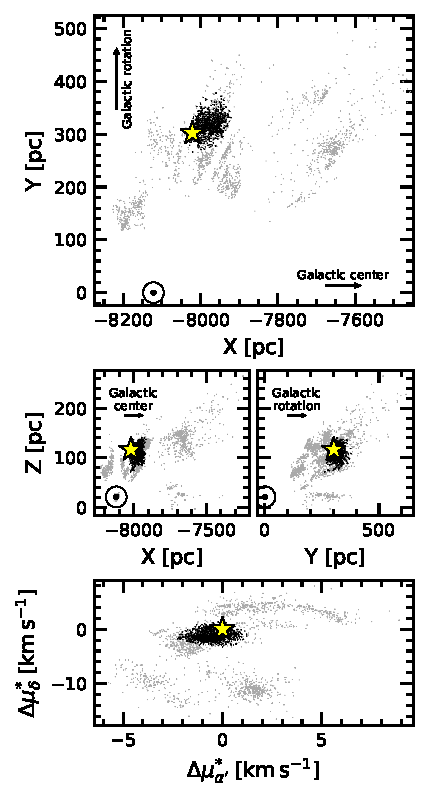
\includegraphics[width=1\textwidth]{f1.pdf}
	\end{center}
	\vspace{-0.7cm}
	\caption{
    {\bf Galactic position and tangential velocities of the
    $\delta$\,Lyr cluster.}
    Points are candidate cluster members with $\varpi/\sigma_\varpi >
    20$, reported to be in the group by
    \citet{kounkel_untangling_2019}.  We focus on stars in a small
    region (black points) in the kinematic vicinity of Kepler\,1627
    (yellow star).  The other candidate cluster members (gray points)
    may or may not share the ages of the selected kinematic group.
    The location of the Sun is ($\odot$) is shown.
		\label{fig:XYZvtang}
	}
\end{figure*}

Figure~\ref{fig:XYZvtang} shows stars reported by
\citet{kounkel_untangling_2019} to be in the group ``Theia 73'', which
was cross-matched by \citealt{kounkel_untangling_2019} as being
``Stephenson 1''.  For our Figure, galactic positions were calculated
and plotted only for stars with parallax signal-to-noise exceeding 20.
The location of the Sun is shown on the plots.  The smattering of
reported cluster members (gray and black points) has a significantly
different structure that the cluster initially identified by
\citet{stephenson_possible_1959} and corroborated by
\citet{eggen_photometric_1968}.  While the non-uniform ``clumps''
might be part of a real structure, they could also be an artifact of
the data processing steps performed by
\citet{kounkel_untangling_2019}.  We therefore opted to only consider
stars in the immediate kinematic and spatial vicinity of \sn.  The
tangential velocities relative to \sn\ are shown in the bottom right
panel.  These are computed by assuming that every star has the same
three-dimensional spatial velocity as \sn, where we assume a systemic
radial velocity of $-16.7 \pm 0.2$\,\kms\ based on the reconnaissance
spectra obtained by A.~Howard on HIRES and D.~Latham on TRES.  The
relevant projection effects are then taken into account, as discussed
by {\it e.g.}, \citet{Meingast2021} and \citet{bouma_2021_ngc2516}.
We performed the actual selection by then manually drawing lassos with
the interactive \texttt{glue} visualization tool
\citep{beaumont_2014_13866} in the four projections shown in
Figure~\ref{fig:XYZvtang}.  While bonafide members likely exist
outside of our selection region (and our selection also includes some
field star interlopers), our aim is to verify the existence of the
cluster in the vicinity of Kepler\,1627, and to measure its age.  The
procedure we have adopted enables both tasks.


\section{Transit and Stellar Variability Model}
\label{app:gptransit}

\subsection{Long Cadence Data}
\begin{figure*}[t]
	\begin{center}
		\leavevmode
		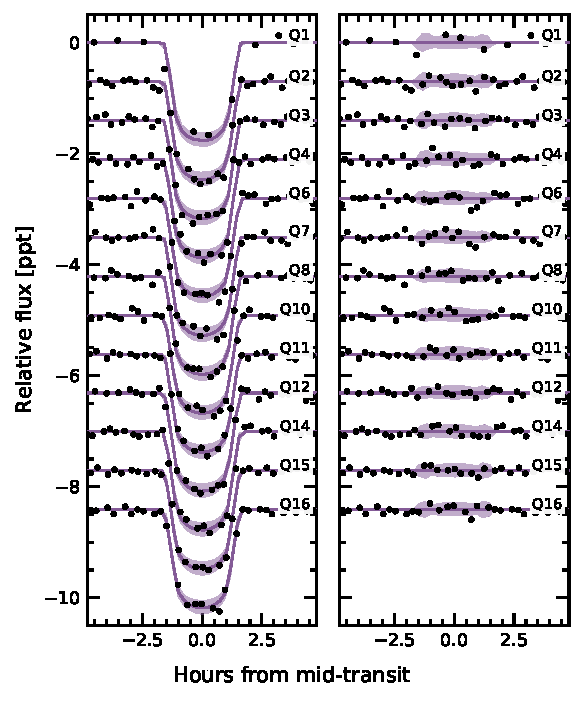
\includegraphics[width=1\textwidth]{f9.pdf}
	\end{center}
	\vspace{-0.7cm}
	\caption{
		{\bf Transit model residuals through time}.  
    {\it Left:}
		Phase-folded transit of Kepler 1627b, with stellar
    variability removed, binned by Kepler quarter.
    Black points are binned to 20 minute intervals.
    The 1-$\sigma$ model uncertainties and the maximum {\it a
    posteriori} model are shown as the faint purple band, and the dark
    purple line.
    {\it Right:}
    As on the left, with the transit removed.
    Quarters 6 and 7 show a consistent deviation in the second half of
    the transit.
		\label{fig:phasequarter}
	}
\end{figure*}

\begin{figure*}[t]
	\begin{center}
		\leavevmode
		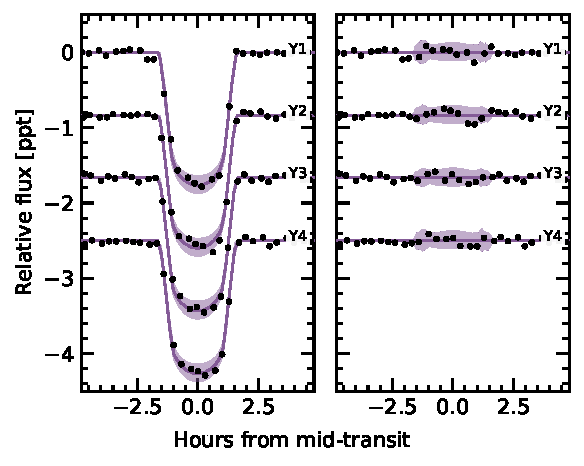
\includegraphics[width=1\textwidth]{f10.pdf}
	\end{center}
	\vspace{-0.7cm}
	\caption{
    {\bf Transit model residuals through time (Part 2)}.  
    {\it Left:}
		Phase-folded transit of Kepler 1627b, with stellar
    variability removed, binned by year of observation.
    Points and models are as in Figure~\ref{fig:phasequarter}.
    {\it Right:}
    As on the left, with the transit removed.
		\label{fig:phaseyear}
	}
\end{figure*}



We assumed a quadratic limb-darkening law, with the uninformative prior
advocated by CITET Kipping2013.

% In the first approach, we adopted uniform priors centered on the
% interpolated CITET Claret+2011 coefficients in the Kepler-band, with
% with $\pm 0.2$ in either parameter.  The fit was not as good.

Our default stellar variability model (RotGPtransit) allows for a
\texttt{RotTerm} GP kernel, with a logjitter term to inflate the
uncertainties to account for excess white noise.  (This results in an
inflation of the uncertainties by a factor of about three).

We considered including an additive \texttt{SHOTerm} kernel to account
for stochastic noise (RotStochGPtransit).  This didn't seem to affect
the results much, so we opted for the simpler model.

Figure~\ref{fig:phasefold} shows X, Y, Z.  The residuals during the
transit may hint at some small degree of unfitted signal -- in the
sense that the observations are systematically high in the first half
of transit, and low in the second half.  This is the phase of maximal
scatter during each orbital period (TODO: in vs out of transit
scatter).  The amplitude of the anomaly is $\approx$30\,ppm.

To explore the origin of the anomaly, we binned the Kepler data over
quarters (Figure~\ref{fig:phasequarter}) and years
(Figure~\ref{fig:phaseyear}).  In Figure~\ref{fig:phasequarter}
Quarter 6 shows the strongest asymmetry out of any of the quarters: a
deviation of about 3\,ppt from expectation.  Quarter 7 shows an
anomaly at roughly the same transit phase.  Year 2 correspondingly
shows the strongest anomaly out of any year in
Figure~\ref{fig:phaseyear}.

We considered three possible explanations for the anomaly: gravity
darkening, transit timing variations, and spot-crossing events.

Gravity darkening (e.g., CITE Masuda 2015) is based on the premise
that the rapidly rotating star becomes oblate, and brighter near the
poles than the equator.  The fractional shape change due to gravity
darkening is on the order of $(P_{\rm break}/P_{\rm rot})^2$, for
$P_{\rm break}$ the break-up rotation period, and $P_{\rm rot}$ the
rotation period.  Using the parameters from Table~\ref{tab:posterior},
this yields an expected 1.6\% distortion of the $\approx$1.8\,ppt
transit depth: {\it i.e.}, an absolute deviation of $\approx$3\,ppm.
This is smaller than the observed anomaly by an order of magnitude,
and therefore seems unlikely.

The scenario of transit timing variations (TTVs) producing the
asymmetry seems unlikely, since the analysis by
\citet{holczer_transit_2016} implies that any such variations in \sn\
need to be less than of order minutes.  Figures~\ref{fig:phasequarter}
and~\ref{fig:phaseyear} also provide little evidence in support of
this possibility.

The final possibility is that of starspot crossings.  Given the high
expected spot-covering fractions for young stars ({\it e.g.},
\citealt{morris_relationship_2020}, \citealt{plavchan_planet_2020}),
\pn\ may cross spot groups on the stellar surface in projection.
Spot-crossing anomalies often reach amplitudes exceeding 100\,ppm
({\it e.g.}, CITE Dai 2018, maybe Southworth's recent stuff).  For our
system,  $P_{\rm orb}/P_{\rm rot} \approx 2.76$.  This means that
every 4 transits (and 11 stellar rotations), the planet crosses over
roughly the same stellar longitude.  Over a given quarter, this could
occur at most three times, assuming the spot groups are persistent.  

This could provide a plausible path to creating the distorted transit
signal, based on the amplitudes involved.  However, the typical S/N
per Kepler transit is $\approx8$, making individual spot-crossing
unresolved, and this scenario challenging to test.  {\it A priori},
one would also expect the spot-crossing events to not have a preferred
orbital phase, so that they would average out over the $\approx200$
Kepler transits.  Nonetheless, given the available data, it is our
best explanation for what we believe is real additional photometric
scatter observed during the transits.

\subsection{Short Cadence Data}

\begin{figure*}[t]
	\begin{center}
		\leavevmode
		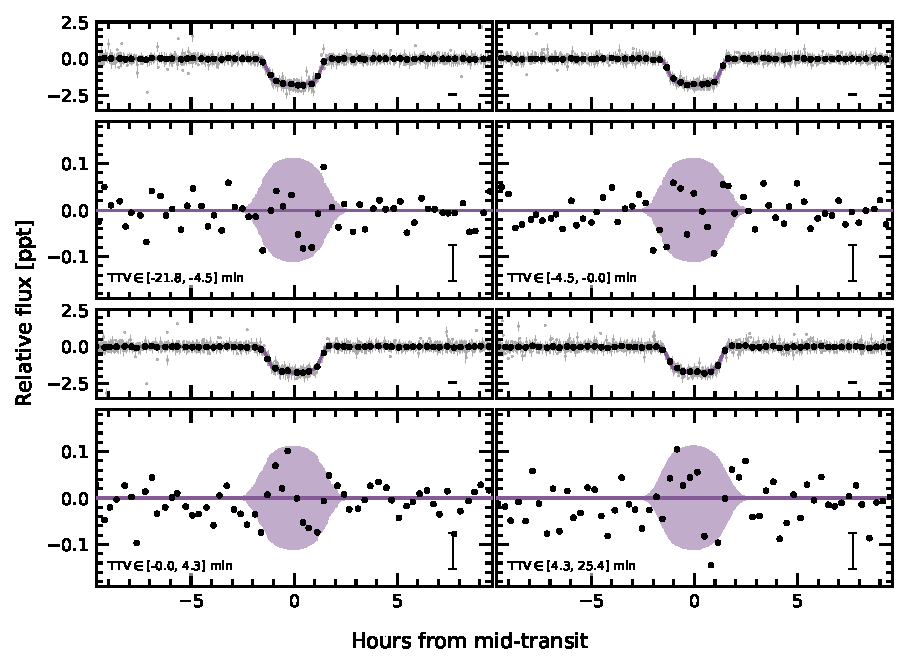
\includegraphics[width=1\textwidth]{f12.pdf}
	\end{center}
	\vspace{-0.7cm}
	\caption{
		{\bf Phase-folded short cadence transit of Kepler\,1627 Ab}.  
    The precision with which the impact parameter can be measured is
    higher than from the long cadence data.
		\label{fig:phase_slc}
	}
\end{figure*}

Figure~\ref{fig:phase_slc} shows the result from analyzing 100 days of
short cadence (1-minute) data acquired during Quarter 15.
%TODO: get quantitative on better impact parameter...





\section{Flare Analysis}
\label{app:flare}

\begin{figure*}[t]
	\begin{center}
		\leavevmode
		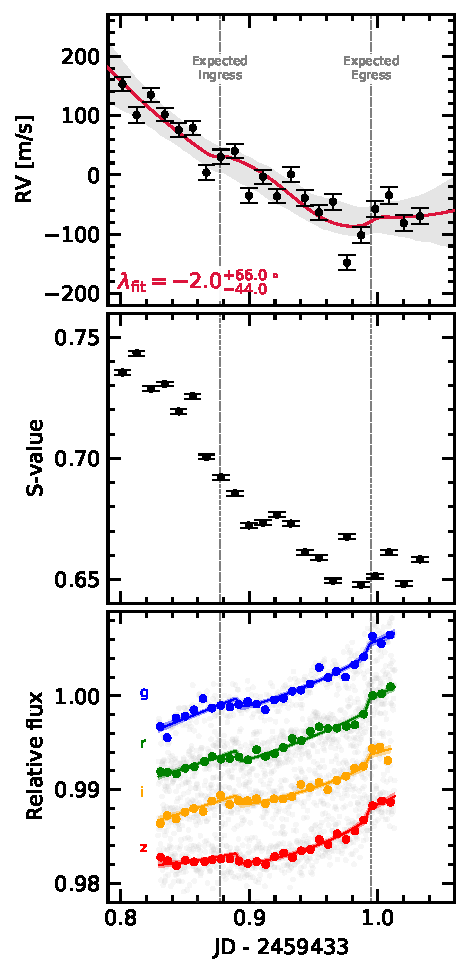
\includegraphics[width=1\textwidth]{f7.pdf}
	\end{center}
	\vspace{-0.7cm}
	\caption{
		{\bf Flares in Kepler\,1627}.  
    {\it Top:}
    The full short-cadence Kepler dataset, acquired at 1-minute
    sampling (black points) is shown with a stellar variability model
    (blue line).
    {\it Middle:}
    Residual after subtracting the stellar variability model.  Flares
    appear as spikes.
    {\it Bottom:}
    Zooms of the brightest, and third-brightest flares.  A timing
    coincidence -- that both flares have ``successors'' approximately
    one orbital period after the initial event -- is emphasized.
		\label{fig:flarezoom}
	}
\end{figure*}

\begin{figure*}[t]
	\begin{center}
		\leavevmode
		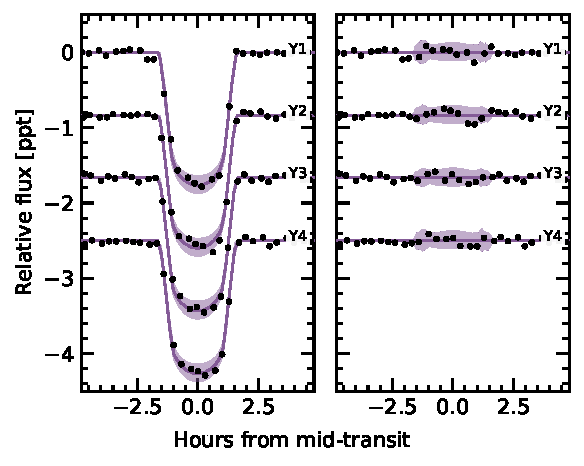
\includegraphics[width=1.0\textwidth]{f8.pdf}
	\end{center}
	\vspace{-0.7cm}
	\caption{
		{\bf Phase-folded flares in Kepler\,1627}.  
    {\it Top:}
    As in the middle of Figure~\ref{fig:flarezoom}, phase-folded at
    the planet's ephemeris.
    {\it Bottom:}
    Fitted flare amplitudes and orbital phases -- each point
    represents one flare.
    Colors indicate relative time, from the beginning of the
    98-day short-cadence Quarter 15 dataset (dark blue) to the end (light
    yellow).
    Lower amplitude flares likely exist in the data, and were not
    examined.
		\label{fig:flarephase}
	}
\end{figure*}

\begin{figure*}[t]
	\begin{center}
		\leavevmode
		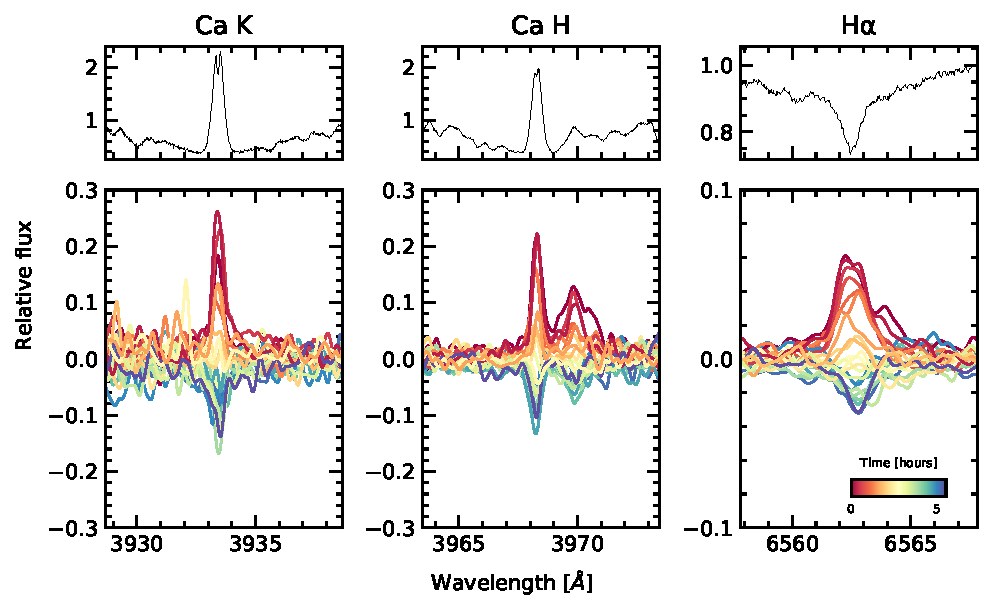
\includegraphics[width=1.0\textwidth]{f13.pdf}
	\end{center}
	\vspace{-0.7cm}
	\caption{
		{\bf Statistics of inter-flare arrival times}.  
    24 flares were recorded with amplitudes exceeding 0.5\% over the
    97.7 days of short cadence observations.  The histogram of the
    time intervals between every possible pair of flares is shown in
    black.  Some plausibly important timescales for star-planet
    interactions, namely the planetary orbital period and synodic
    period (the orbital period as seen from the rotating stellar frame) are
    shown along with their linear combinations.  Monte Carlo
    draws from a Poisson distribution are shown
    with the gray bands.  While peaks in the observed distribution do
    coincide with the locations of these ``special periods'', the
    statistical evidence for a non-Poissonian process driving the
    flares does not reach the $5$-$\sigma$ threshold.
		\label{fig:flarestats}
	}
\end{figure*}

The short cadence (1-minute) Kepler observations span 97.7 days.
The light curve shows a significant number of flares
(Figure~\ref{fig:flarezoom}).
To quantify clean the light curve and identify the flares, we
performed the following procedure.
For cleaning, we performed the following iterative detrending procedure.
\begin{itemize}
  \item Step 1: Build a two-term mixed SHOTerm GP model with
    quasi-periodic kernels at Prot and 0.5$\times$Prot. Fit the model
    to the time, flux, and flux uncertainty.
  \item Step 2: Select points more than twice the median absolute
    deviation from the residual, and exclude them from the light
    curve.  Repeat Step 1.
  \item Step 3: On the residual from Step 2, identify all flares,
    requiring them to be at least 20 cadences apart, at least 7 median
    absolute deviations above the median baseline, and lasting at least
    2 cadences in duration.  Build the mask spanning these times, from
    5 minutes before each flare begins to 2.5 minutes after the final
    flare cadence.  Repeat Step 1 a final time.
\end{itemize}
The flares were then identified and fitted using ALTAIPONY (CITE CITE).
The fitted model is that of CITE XXX, which parametrizes the flare
with a start time, a lag time, and an amplitude (CHECK).
Figure~\ref{fig:flarephase} shows the resulting flares, amplitudes,
and phases.

There were $N_{\rm f}=24$ flares exceeding $0.5\%$ in relative flux during the
short-cadence observations.  These 24 flares spanned a total of 6.5
hours ($\sim$15 minutes per flare).  For better or worse, we noticed a
coincidence in the flare arrival times.  The coincidence is that
despite the low flare duty cycle, one orbital period after the
brightest flare, a second flare followed.  This and a similar event
are shown in Figure~\ref{fig:flarezoom}.  The timing error is good to
a $\approx0.2\%$ difference from the orbital period, which seems {\it
a priori} unlikely.  If we consider flares falling within 2\% of the
planet's orbital period after a previous flare, then 4 of the 24 flare
events have candidate ``successors''.

As with any coincidence, when one does not have a firm prediction, it
is difficult to assess the statistical significance of a surprise.
Since our surprise was specifically at the inter-arrival time of
certain flares coinciding with special time intervals, we performed
the following analysis.  First, we considered all unordered pairs of
flares.  For $N$ flares there are ${n \choose 2}$ such pairs (for our
case, 276 pairs).  We then compared the distribution of the pair
separations against that from a Poisson distribution.  Specifically,
we drew $N_{\rm f}=24$ samples from a Poisson distribution with
$\lambda = \Delta t / N_{\rm f}$, for $\Delta t=97.7\,{\rm days}$ the
duration of the observations, and repeated the draw $10^3$ times with
unique random seeds.

Figure~\ref{fig:flarestats} shows the results.  The vertical lines in
the figure show the planetary orbital period, the synodic period
$P_{\rm syn} = (P_{\rm rot}^{-1} - P_{\rm orb}^{-1})^{-1}$, and linear
combinations thereof.  Note that the tidal period (half the synodic
period) is not shown.  The bins are logarithmically spaced to give 100
bins between the minimum and maximum ordinate values.  The gray bands
express the range of values observed from the Poissonian draws.  While
it does seem like a rather odd coincidence for peaks in the observed
flare arrival time distribution to coincide with the locations of
these ``special intervals'', the statistical evidence for a
non-Poissonian process driving the flares does not seem particularly
strong.  More quantitatively, the peaks observed at the orbital and
synodic periods are within the $\pm 2$-$\sigma$ range of a
Poissonian process, and those at $P_{\rm orb}+P_{\rm syn}$ and $P_{\rm
orb}+2P_{\rm syn}$ are only slightly above this range. 
With that said,
future analyses of these data by investigators more versed in the
topic than ourselves could very well yield new insights.



\section{Companion Star and False Positive Assessment}
\label{app:companionstar}

\begin{figure*}[t]
	\begin{center}
		\leavevmode
		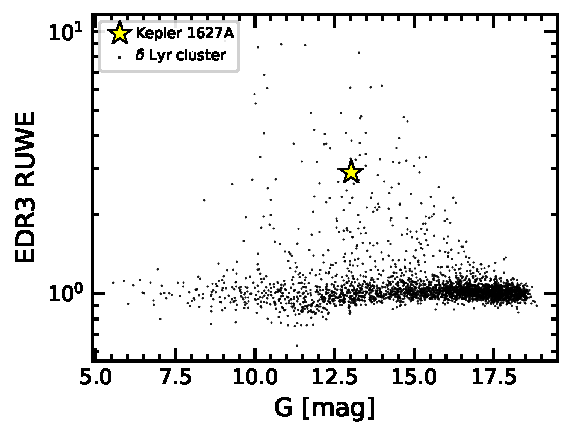
\includegraphics[width=0.6\textwidth]{f6.pdf}
	\end{center}
	\vspace{-0.7cm}
	\caption{
    {\bf Gaia EDR3 renormalized unit weight error (RUWE) point
    estimates for Kepler\,1627A and other members of
    the $\delta$\,Lyr cluster.}  Since other members of the cluster
    with similar colors have comparable degrees of photometric
    variability, the high RUWE estimate suggests that Kepler\,1627A is
    a binary. 
		\label{fig:ruwe}
	}
\end{figure*}

\begin{figure*}[t]
	\begin{center}
		\leavevmode
		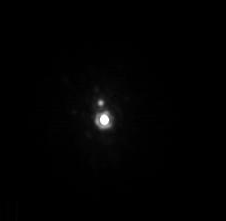
\includegraphics[width=0.6\textwidth]{TEMP_binarity_ao.png}
	\end{center}
	\vspace{-0.7cm}
	\caption{
    {\bf Keck NIRC2 AO image of Kepler 1627A and Kepler 1627B.}  
    {\bf SCALEBAR DENOTES...}
    {\bf North is up, East is left}.
    \label{fig:ao}
	}
\end{figure*}

Our analysis of archival Keck-NIRC2 Kp-band (2.12\,$\mu $m) imaging
revealed the existence of a previously unreported stellar neighbor,
unresolved in the Gaia source catalog {\bf FIXME: uncertainties}.  The
NIRC2 images yield a projected separation $\rho=0\farcs17$, with
$\Delta {\rm Kp} = 2.5$.  Using the measured Gaia EDR3 parallax for
the system, this implies a projected separation of 54\,AU.  The
presence of this star is consistent with the excess noise in the Gaia
astrometric time-series (see Section~\ref{app:companionstar}).  Given
the low chance of a star imaged within {\bf X.X arcseconds} to be a
chance companion along the line of sight, we proceed under the
assumption that it is bound, and that the Kepler\,1627 system is
binary.

Unforuntately, we do not have any reliable color information about
Kepler\,1627B.  Based on the
tabulation\footnote{\url{http://www.pas.rochester.edu/~emamajek/EEM_dwarf_UBVIJHK_colors_Teff.txt},
version \texttt{2021/03/02}.} by \citet{pecaut_mamajek_2013}, the
measured NIR-contrast for a main sequence G8V star corresponds to a
spectral type for the companion of $\approx$M2V ($M_\star \approx
0.44\,M_\odot$).  However, the companion should have a longer
pre-main-sequence contraction phase than the primary, which would
imply that this mass is overestimated by $\sim10$ to $20\%$.

Could the companion be creating a false positive signal?  The
companion star contributes $\approx$1\% of the total flux observed in
the Kepler aperture (0.7-2.0\% V-band to G-band dmag difference from
EEM table; todo is fix using model spectra).  The observed transit has
a depth of 0.18\%.  An 18\% deep eclipse of the secondary star would
therefore be needed to produce a deep enough signal.  The shape of the
observed signal requires allowed impact parameters to span 0.02 to
0.73 (Table~\ref{tab:posterior}); the body transiting the secondary
would therefore need to be non-grazing with $R_3/R_2 \approx 0.42$.
Assuming a $\approx 0.42R_\odot$ radius of the imaged secondary, this
would imply a tertiary stellar radius of $\approx 0.2R_\odot$.  This
scenario ultimately yields a contradiction, because it would require
an ingress and egress phase that each span $\approx$40\% of the
transit duration ($\approx 65\,{\rm minutes}$).  The actual measured
ingress and egress duration is $\approx 15\,{\rm minutes}$),
4.4$\times$ shorter.

\paragraph{Stellar density implied by transit duration}
The duration of the transit ($2.823 \pm 0.057 hr$) and the implied
stellar density ($2.31 \pm 0.52\,{\rm g\,cm}^{-3}$) could in theory
help rule between whether the transiting body orbits the primary or
secondary star.  Ultimately, our stellar density measurement is not
precise enough to render the blend scenario implausible.  At 30 Myr, a
0.40\,$M_\odot$ solar-metallicity dwarf is $\approx 26\%$ larger than
when it is fully contracted on the main sequence (0.40\,$R_\odot$
vs{.} 0.50\,$R_\odot$; CITEALT: Choi et al, MIST grids).  The
theoretically implied companion density of $3.2\,{\rm g\,cm}^{-3}$ is
indeed larger than the primary star's density of $1.80\,{\rm
g\,cm}^{-3}$ (measured through the HIRES reconaissance spectroscopy).
However the stellar density measured from the transit fitting ($2.31
\pm 0.52\,{\rm g\,cm}^{-3}$) is only discrepant at the
$\approx$2-$\sigma$ level from the M-dwarf blend scenario.  It is
instead the combination of the flux contrast, transit depth, and
ingress duration that rule out this scenario.









% \section{Bonus figures that wont be included}
% 
% \begin{figure*}[t]
% 	\begin{center}
% 		\leavevmode
% 		\includegraphics[width=1\textwidth]{dontinclude0.png}
% 	\end{center}
% 	\vspace{-0.7cm}
% 	\caption{
%     {\bf corner plot of gptransit fit}
% 	}
% \end{figure*}


\listofchanges

%\allauthors
\end{document}
